% !TEX root =  main.tex
\chapter{The Classroom as a PCA}
\hspace{\parindent} The classroom is a complex system that can be modeled as a probabilistic cellular automata (PCA). 
This chapter will discuss the classroom as a complex system and the probabilistic cellular automata model. 
The chapter will also discuss the implications of the model on the classroom and the teaching-learning process. 
(AI Generated Text)

Probably add objectives here???

\section{Cellular Automata and its use in modelling complex systems}

A two-dimensional (2D) rectangular cellular automata can be defined by a five-tuple \cite{arciaga2009experimental} + Reinier MS:

\begin{equation}
    \label{eq:CA definition}
    \text{CA} = \lbrace \mathcal{S,C,L,N,R} \rbrace
\end{equation}

where
\newlist{CAdef}{itemize}{1}
\newcommand\itemS{\item[$\mathcal{S}=$]}
\newcommand\itemC{\item[$\mathcal{C}=$]}
\newcommand\itemL{\item[$\mathcal{L}=$]}
\newcommand\itemN{\item[$\mathcal{N}=$]}
\newcommand\itemR{\item[$\mathcal{R}=$]}

\begin{CAdef}
    \itemS is the set of possible states that each cell can assume. The state $s$ can use any kind of representation such as the set of integers $\lbrace 0,\ldots,n-1\rbrace$ with $n$ as the total number of possible states.
    
    \itemC $\lbrace c = {i,j} \mid i \in \lbrace 1,2,3,\dots,L_1 \rbrace, j \in \lbrace 1,2,3,\dots,L_2\ \rbrace \text{s.t. } L_1 \times L_2 = N \rbrace$ is the set of identifiers for each cell in the automaton where $N$ is the total number of cells and $L_1$ and $L_2$ are the lengths of each side of the automaton space. The cells can then be identified by their position in the automaton $(i,j)$. So, the state of cell $c \in \mathcal{C}$ can be written as $s_c = s_{i,j} \in \mathcal{S}$
    
    \itemL defines the lattice neighborhood which is generally a mapping $f : \mathcal{C} \rightarrow C^M$ where $M$ is the number of neighbors of a cell $c \in \mathcal{C}$. Any given cell $c$ is mapped to another tuple of cells: $L_{i,j} = \lbrace (i-1,j-1), (i-1, j), (i-1, j+1), (i, j-1), \dots, (i,j)$. Where $r$ is the radius of the Moore neighborhood. We then say that $\mathcal{L}_{i,j}$ contains the set of neighboring cell for $c_{i,j}$.
    
    \itemN $\mathcal{S}^M$, the set of neighborhood states. Thus, $N_c = N_{i,j} \in \mathcal{N}$ such that each $\mathcal{N}$ is in the form of the $M$-tuple $\lbrace s_{i-1,j-1}, s_{i-1, j}, s_{i-1. j+1}, s_{i, j-1}, \dots, s_{i,j} \rbrace$.
    
    \itemR defines the set of rules implemented in the CA with $g : s_{i,j} \mid \mathcal{L} \rightarrow \mathcal{S}$ as the mapping of any neighborhood state $N_c$ to a new state $s'_{i,j}$ of the cell $c$. At the next time step, $s'_{i,j}$ replaces the original state $s_{i,j}$.
\end{CAdef}

$\mathcal{N}$ can vary with the neighborhood structure and the boundary conditions of the automaton. 
The neighborhood structure dictates the shape the neighborhood in the lattice. 
Common neighborhood structures include the von Neumann (diamond) and Moore (square) neighborhoods. 
Boundary conditions dictate how the automaton treats cells at the egde of the lattice when determining the neighborhood. 
Common boundary conditions include toroidal, spherical, and fixed boundary conditions. 

$\mathcal{R}$ can also be affected by other factors such as whether the rules are deterministic or probabilistic and whether they are implemented synchronously or asynchronously. 
An automaton with deterministic rules will always produce the same output given the same input, while an automaton with probabilistic rules will produce different outputs given the same input. 
In Conway's Game of Life, a cell dies when it has three live neighbors, while a cell is born when it has two or three live neighbors. 
This is an example of a deterministic rule. An example of a probabilistic rule would be a cell dying with a probability of $0.25$ when it has three live neighbors. 
An automaton with synchronous rules will update all cells simultaneously, while an automaton with asynchronous rules will update cells one at a time. 
(something explanation something about sync vs async)


Due to the flexibility of cellular automata, they can be used to model a wide variety of complex systems.
 Cellular automata have been used to model physical systems such as fluid dynamics, biological systems such as the spread of diseases, and social systems such as traffic flow \cite{louis2018probabilistic}.
  Its discreteness and locality make it a good model for systems that are composed of many interacting parts.
   Thus, we have chosen to use a two-state probability cellular automata to simulate the learning process for students in the classroom


\section{PCA model for classroom dynamics}
We used a two-dimensional binary probabilistic cellular automata (PCA) model to simulate the learning process in a classroom. 
In this PCA model, each cell in the automaton represents a student and the state of each cell represents their aptitude $S=\lbrace\text{unlearned, learned}\rbrace=\lbrace 0,1 \rbrace$. 
We assign the neighborhood to be an outer-totalistic Moore neighborhood of radius $r=1$ and define the boundary conditions to be fixed wherein the grid does not wrap around itself and $s_{i,j} = 0$ for ${i,j \notin [1,L]}$. 
How the aumaton updates varies on the learning set up of the classrom. In this study we tackle two learning set ups: traditional and peer instruction (PI). 
We take the traditional instruction to be the case where the teacher is the only source of information for the students - which is typical for classes where the time is mostly spent on lectures. 
In the PI set up, we consider that the students learn from each other but only when the students of interest already know the lesson or is in the learned state.

\subsection{Traditional}
To model the learning process in the traditional classroom, we set the probability for the student to learn in each time $P_{ij}$ to be dependent only on their individual learning rates $\lambda_{i,j}$, which describes how receptive they are to learning, and the probability for the student to learn from the teacher $\rho_0$.

\begin{equation}
    \label{eq:BPCA traditional learning probability}
        P_{ij} = \lambda_{ij} \rho_{0}
\end{equation}

where

$P_{i,j} \in [0,1]$ is the probability of student $c_{i,j}$ to learn in each time step, 

$\lambda_{i,j} = 1$ is the learning rate of student $c_{i,j}$

$\rho_{0} \in [0,1]$ is the probability of $c_{i,j}$ to learn from the teacher

In five-tuple form, the traditional PCA model for the classroom can be written as:

\begin{CAdef}
\itemS $\lbrace \text{learned, unlearned} \rbrace = \lbrace 0, 1 \rbrace$

\itemC $\lbrace (1,1), (1,2), \dots, (1,L), (2, 1), (2,2), \dots, (2,L), \dots, (L,L)\rbrace$ where L is the length of the square classroom.

\itemL $f(c) \leftarrow \lbrack L_c = \lbrace (i+\delta i,j+\delta j) ~\forall~ (\delta i \land \delta j),  \delta i, \delta j \in \lbrace -1,0,1 \rbrace \rbrace $ as a mapping for outer-totalistic Moore neighborhood of radius $r=1$ with a fixed boundary condition.

\itemN $\lbrace 00000000, 00000001, \dots, 11111111 \rbrace$ such that the representation of the neighborhood state $N_c \in \mathcal{N}$ is equivalent to $N_c = \lbrace s_{i+\delta i, j+\delta j} \forall \delta i, \delta j \in \lbrace -1,0,1 \rbrace \rbrace$.

\itemR the probabilistic rule defined by equation \ref{eq:BPCA traditional learning probability}.
\end{CAdef}

The numerical procedure is outlined in Figure \ref{fig:2DBPCA Traditional Flowchart}. Each simulation for the traditional model starts with all students unlearned. The simulation is considered finished once all the students have learned.

\begin{figure}[htbp!]
    \centering
    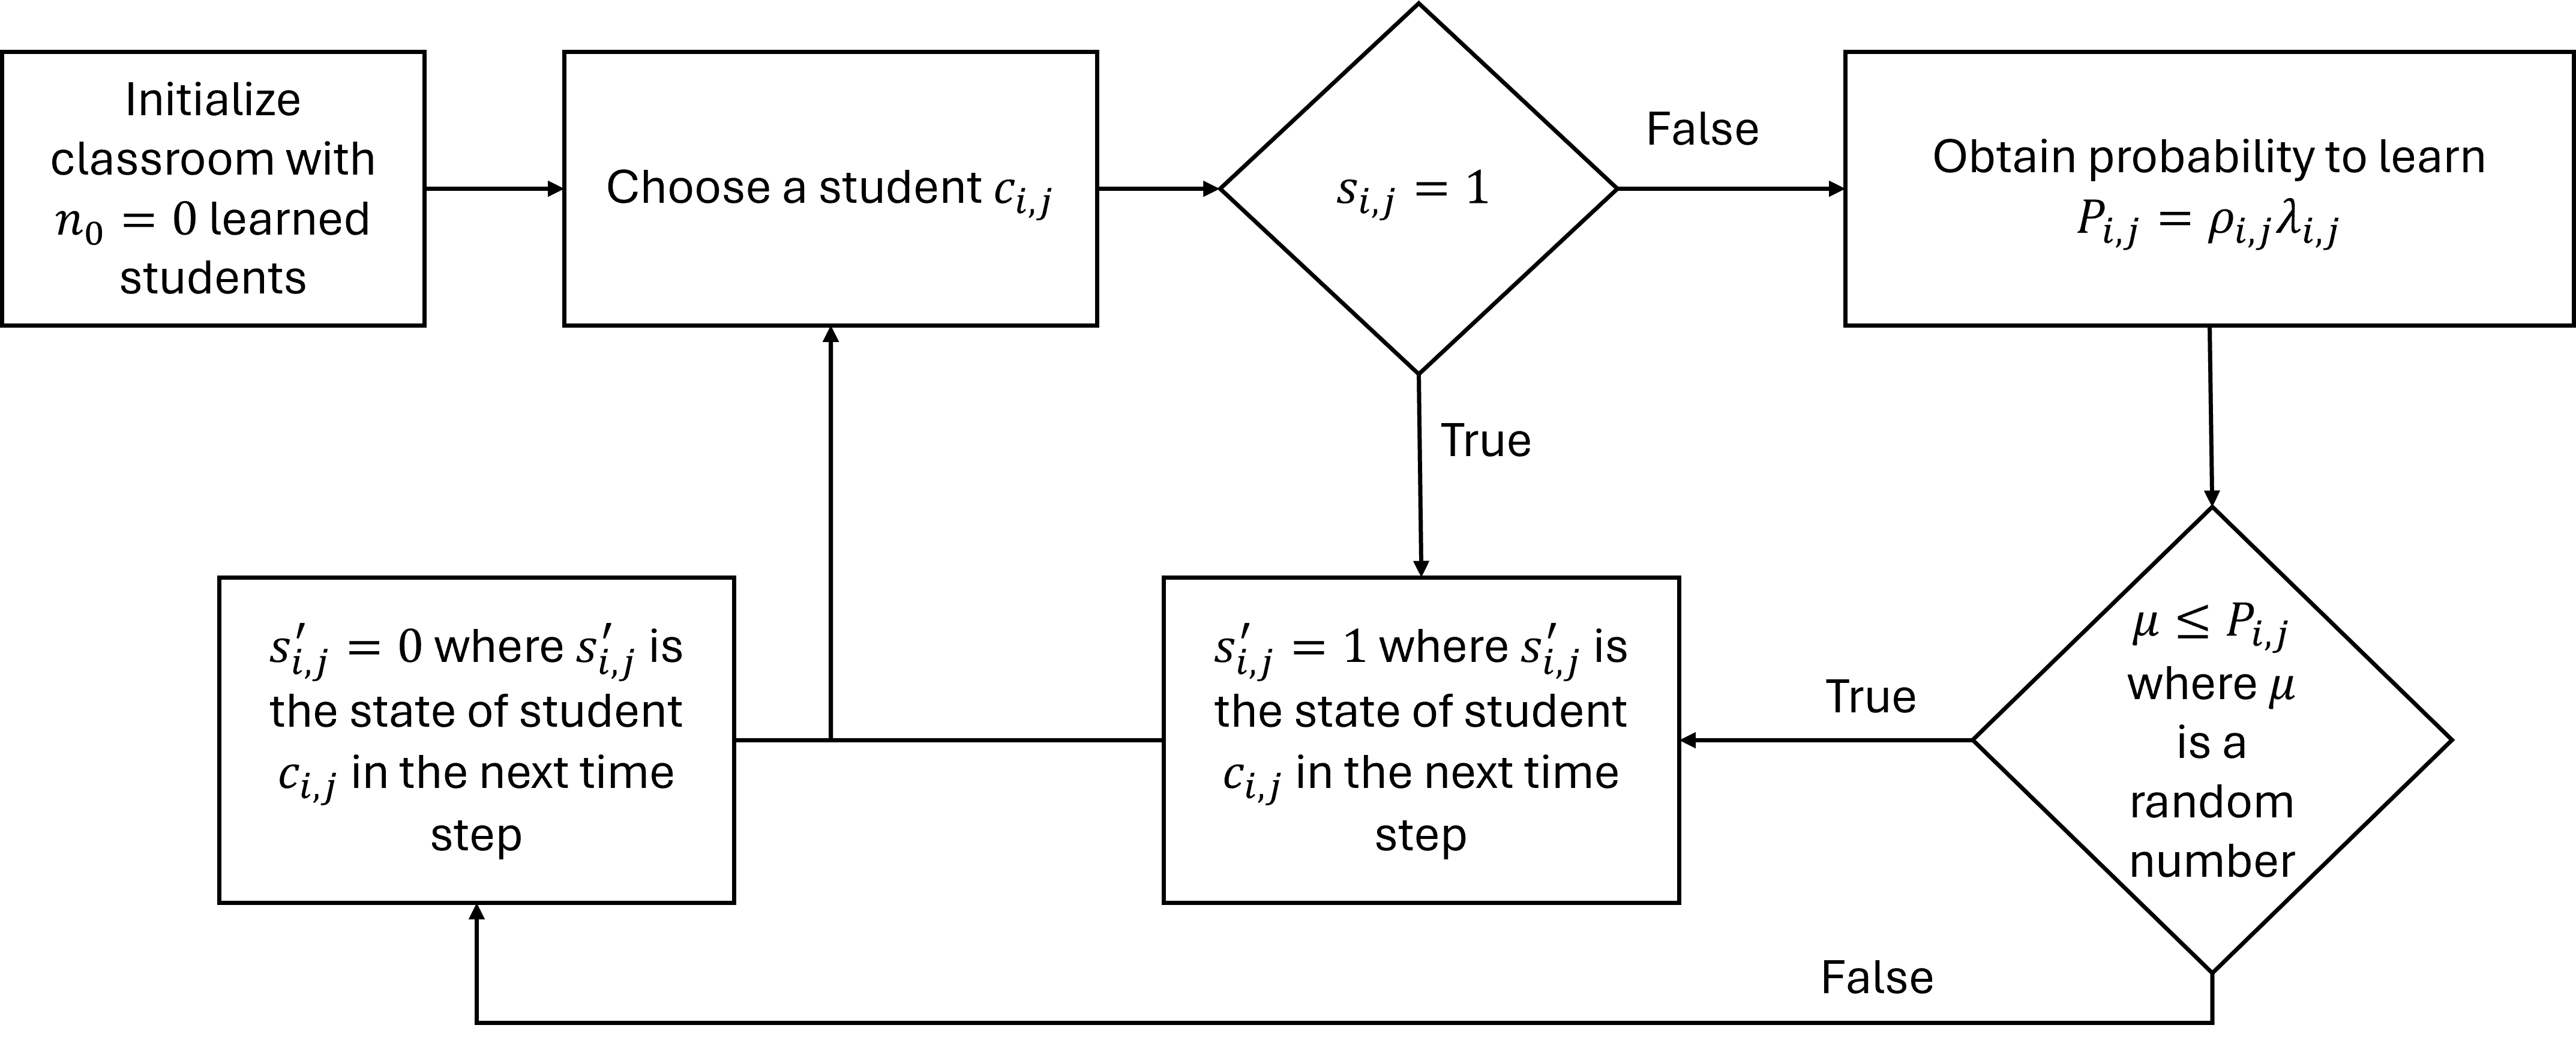
\includegraphics[width=0.8\textwidth]{figures/2DBPCA TI Flowchart.png}
    \caption[Traditional instruction flowchart]{Numerical process for simulation of 2D BPCA for traditional set-ups.}
    \label{fig:2DBPCA Traditional Flowchart}
\end{figure}

\textbf{(figure)} shows an example of a classroom's evolustion over time in the traditional set up. The sample classroom is set with $L=64$, $\lambda_0 = 1$, and $\rho_0 = 0.5$.

\subsection{Peer instruction (PI)}
To model the learning process in a PI set up, we set the probability for the student to learn in each time $P_{ij}$ to be dependent on three factors.
First (1), their learning rate $\lambda_{i,j}$. 
Secondly (2), the positional learning factor $\rho_{i+\delta i, j+\delta j}$ which describes how likely it is to learn from the neighbor $c_{i+\delta i, j+\delta j}$ based solely on their relative position with respect to $c_{i,j}$. 
Lastly (3), the aptitude level of the neighbor $s_{i+\delta i, j+\delta j}$ which dictates whether student $c_{i,j}$ can learn from them. 
The probability for a student to learn in each time step is then determined by the following equation:

\begin{equation}
    \label{eq:BPCA PI learning probability}
        P_{ij} = 1 - \prod_{\forall \delta i, \delta j}{\lbrack1-(\lambda_{ij})(\rho_{i+\delta i, j+\delta j})(s_{i+\delta i, j+\delta j})}\rbrack
\end{equation}

where

$P_{i,j} \in [0,1]$ is the probability of student $c_{i,j}$ to learn in each time step, 

$\lambda_{i,j} = 1$ is the learning rate of student $c_{i,j}$

$\rho_{i+\delta i, j+\delta j} \in [0,1]$ is the probability of $c_{i,j}$ to learn from their neighbors in seats $\lbrace c_{i+\delta i, j+\delta j} \forall \delta i, \delta j \in \lbrace -1,0,1 \rbrace \rbrace$ solely based from their relative positions with each other, and

$s_{i+\delta i, j+\delta j} = \lbrace\text{unlearned, learned}\rbrace=\lbrace 0,1 \rbrace$ are the neighbors' aptitude level.

The derivation of Equation \ref{eq:BPCA PI learning probability} is shown in Appendix \ref{sec: BPCA PI learning probability derivation}.
% \subsection*{spacing? idk}
%\newpage

The numerical procedure is outlined in Figure \ref{fig:2DBPCA PI Flowchart}. 
Each simulation starts the classroom with four learned students $n_0 = 4$ placed in different seats in the classroom. 
The simulation is considered finished once all the students have learned.

\begin{figure}[htbp!]
    \centering
    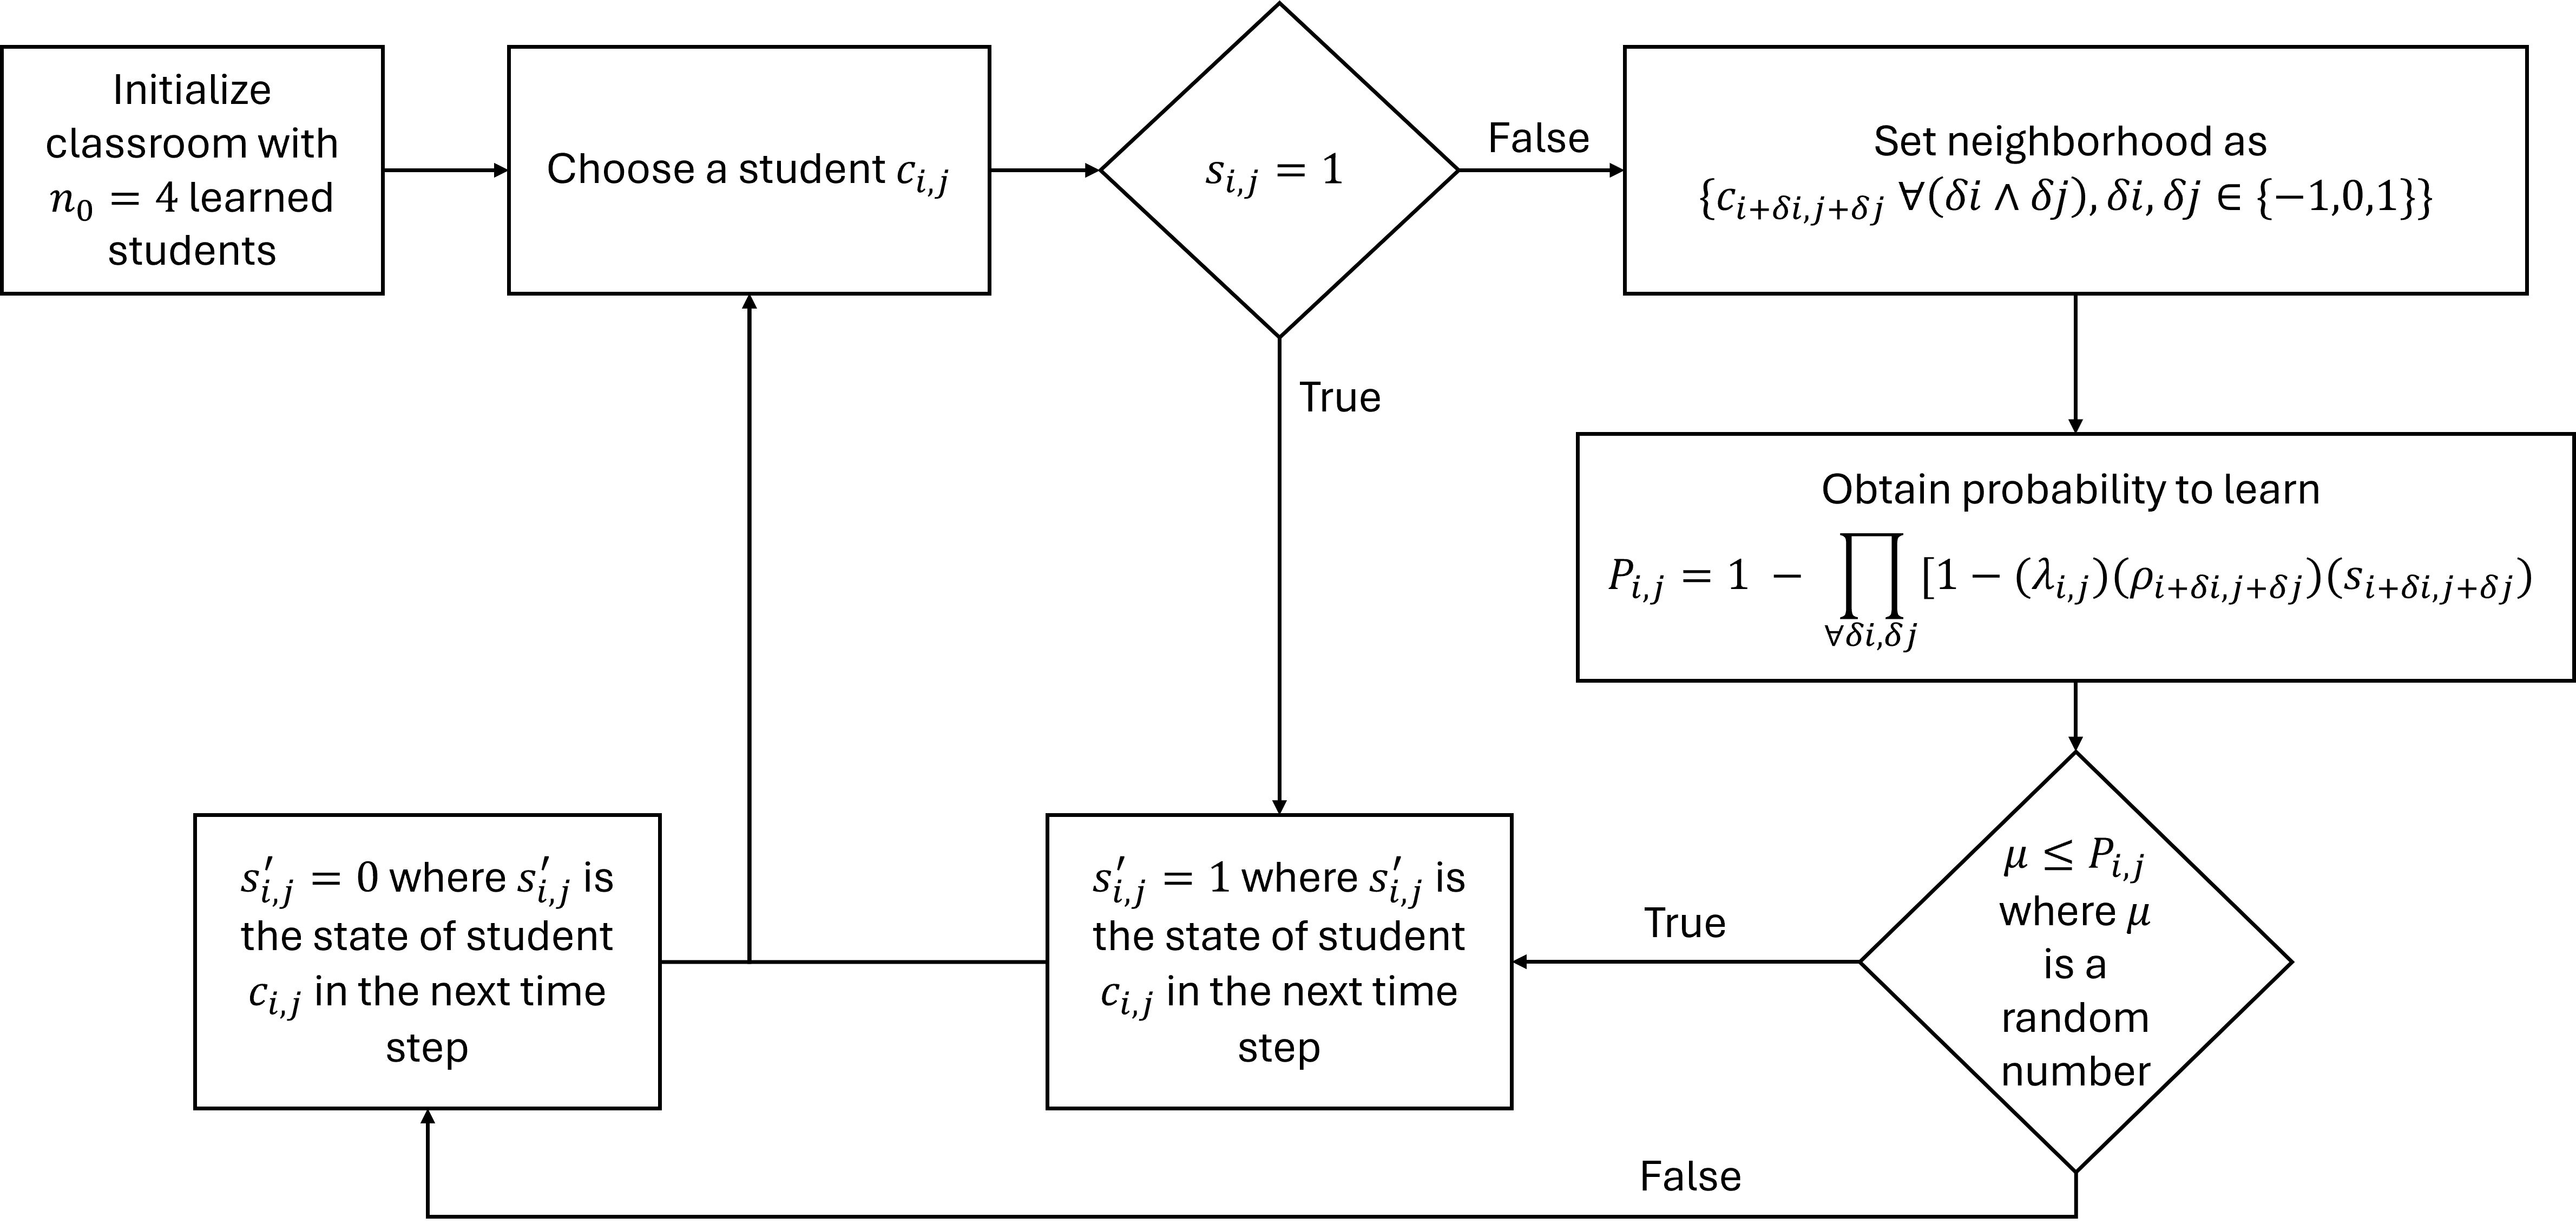
\includegraphics[width=0.8\textwidth]{figures/2DBPCA PI Flowchart.png}
    \caption[Peer instruction flowchart]{Numerical process for simulation of 2D BPCA for PI set-ups.}
    \label{fig:2DBPCA PI Flowchart}
\end{figure}

The seating arrangement (SA) were chosen from a previous study that shows that the SA can affect the learning process \cite{roxas2010seating}. 
These SA's are namely: inner corner, outer corner, center, and random. The SA configurations are shown in Figure \ref{fig:PI SAs}.

 \begin{figure}[htbp!]
    \centering
    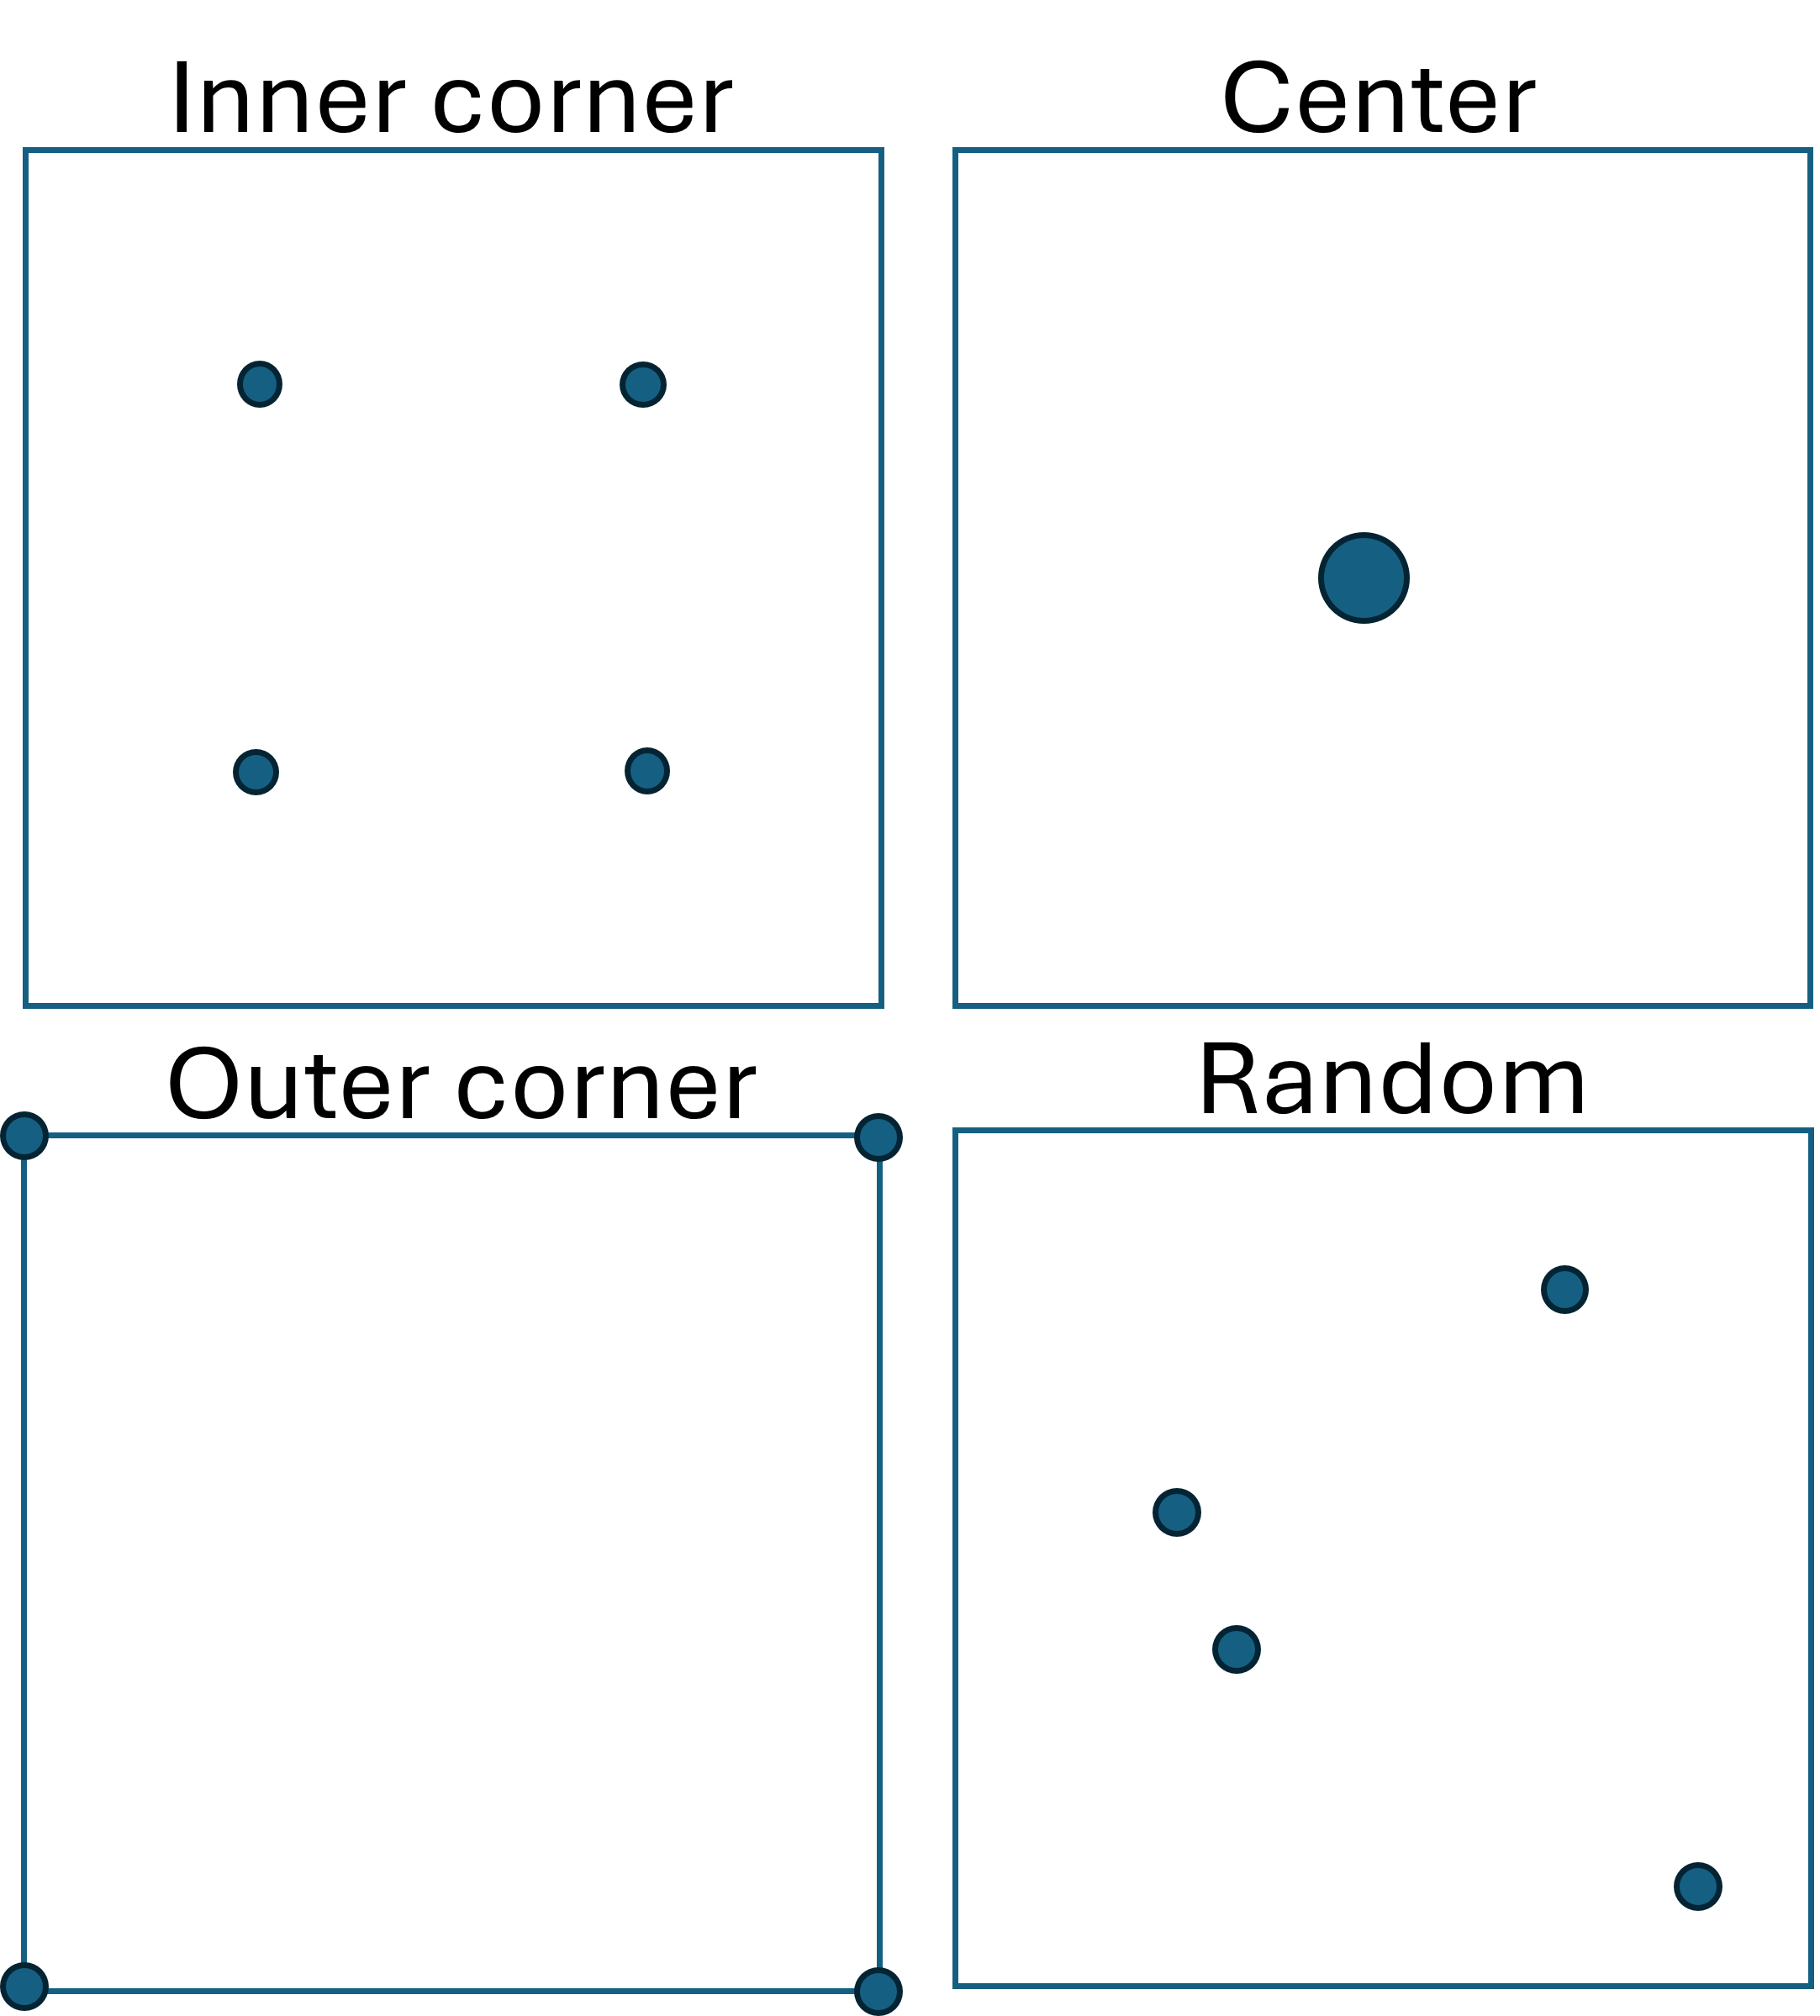
\includegraphics[width=0.5\textwidth]{figures/PI SAs.png}
    \caption[Peer instruction seating arrangements.]{ Peer instruction seating arrangements. 
    Circles denote high aptitude students. 
    The inner corner configuration places high aptitude students halfway between the center and the corner of the classroom. 
    The outer corner configuration places high aptitude students at the corner of the classroom. 
    The center configuration places high aptitude students in the center of the classroom. 
    The random configuration places high aptitude students randomly throughout the classroom.}
    \label{fig:PI SAs}
 \end{figure}

 Figure \ref{fig:Sample classroom evolution} shows an example of classroom's evolution over time. The sample classroom is set with $L=64$, $\lambda_0 = 1$, and $\rho_0 = 0.5$ with the inner corner SA.

 \begin{figure}[htbp!]
    \centering
    \subfigure[$t=1$]{\label{fig:2DBPCA classroom 1}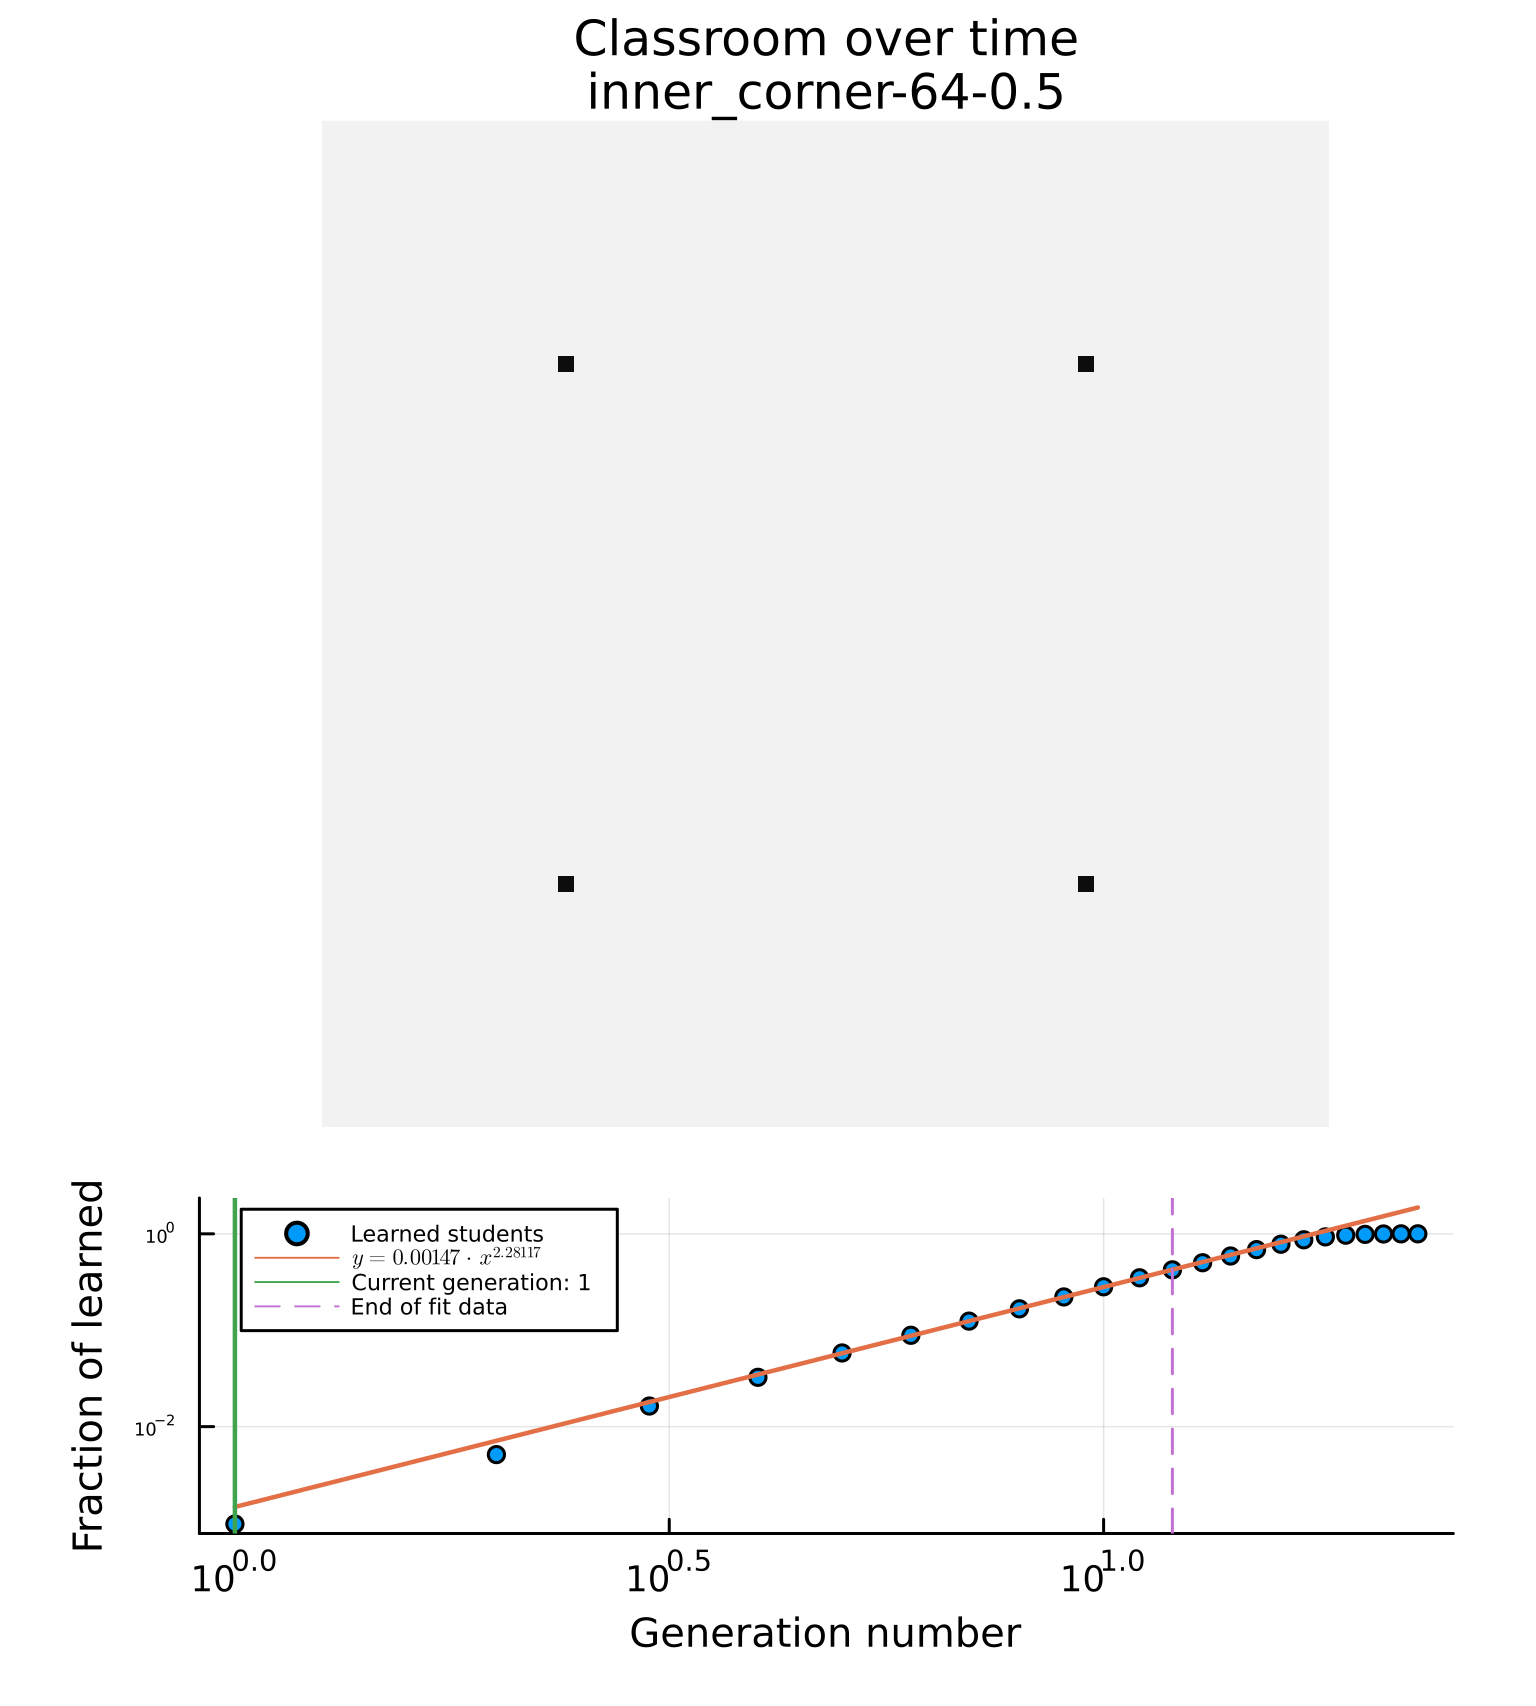
\includegraphics[width=0.45\textwidth]{figures/2D-BPCA-analysis/sample run - PI/2DBPCA-random-64-0.5-1.png}}
    \subfigure[$t=9$]{\label{fig:2DBPCA classroom 9}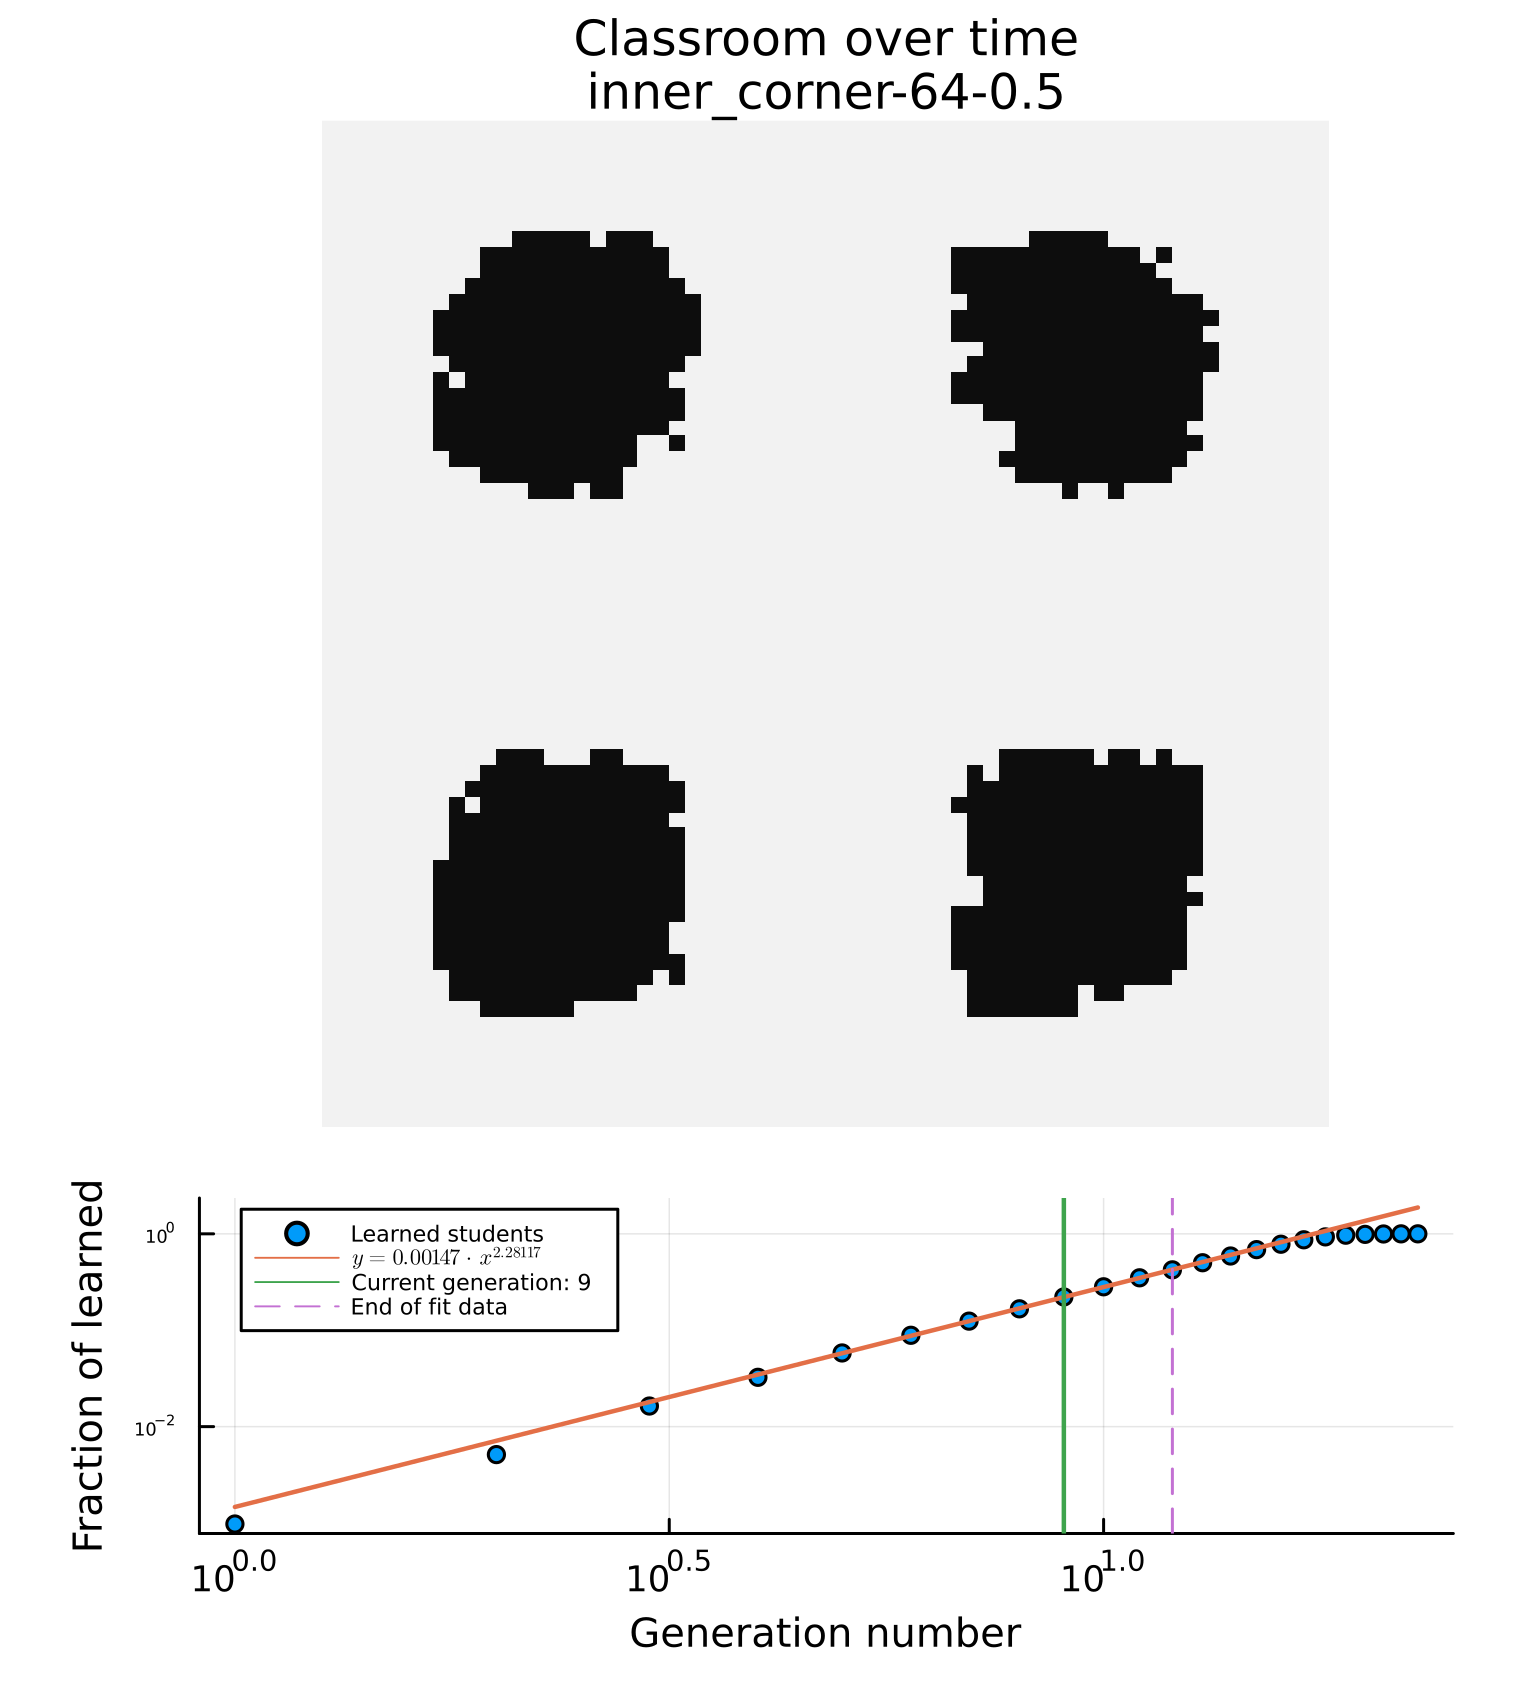
\includegraphics[width=0.45\textwidth]{figures/2D-BPCA-analysis/sample run - PI/2DBPCA-random-64-0.5-9.png}}
    \subfigure[$t=17$]{\label{fig:2DBPCA classroom 17}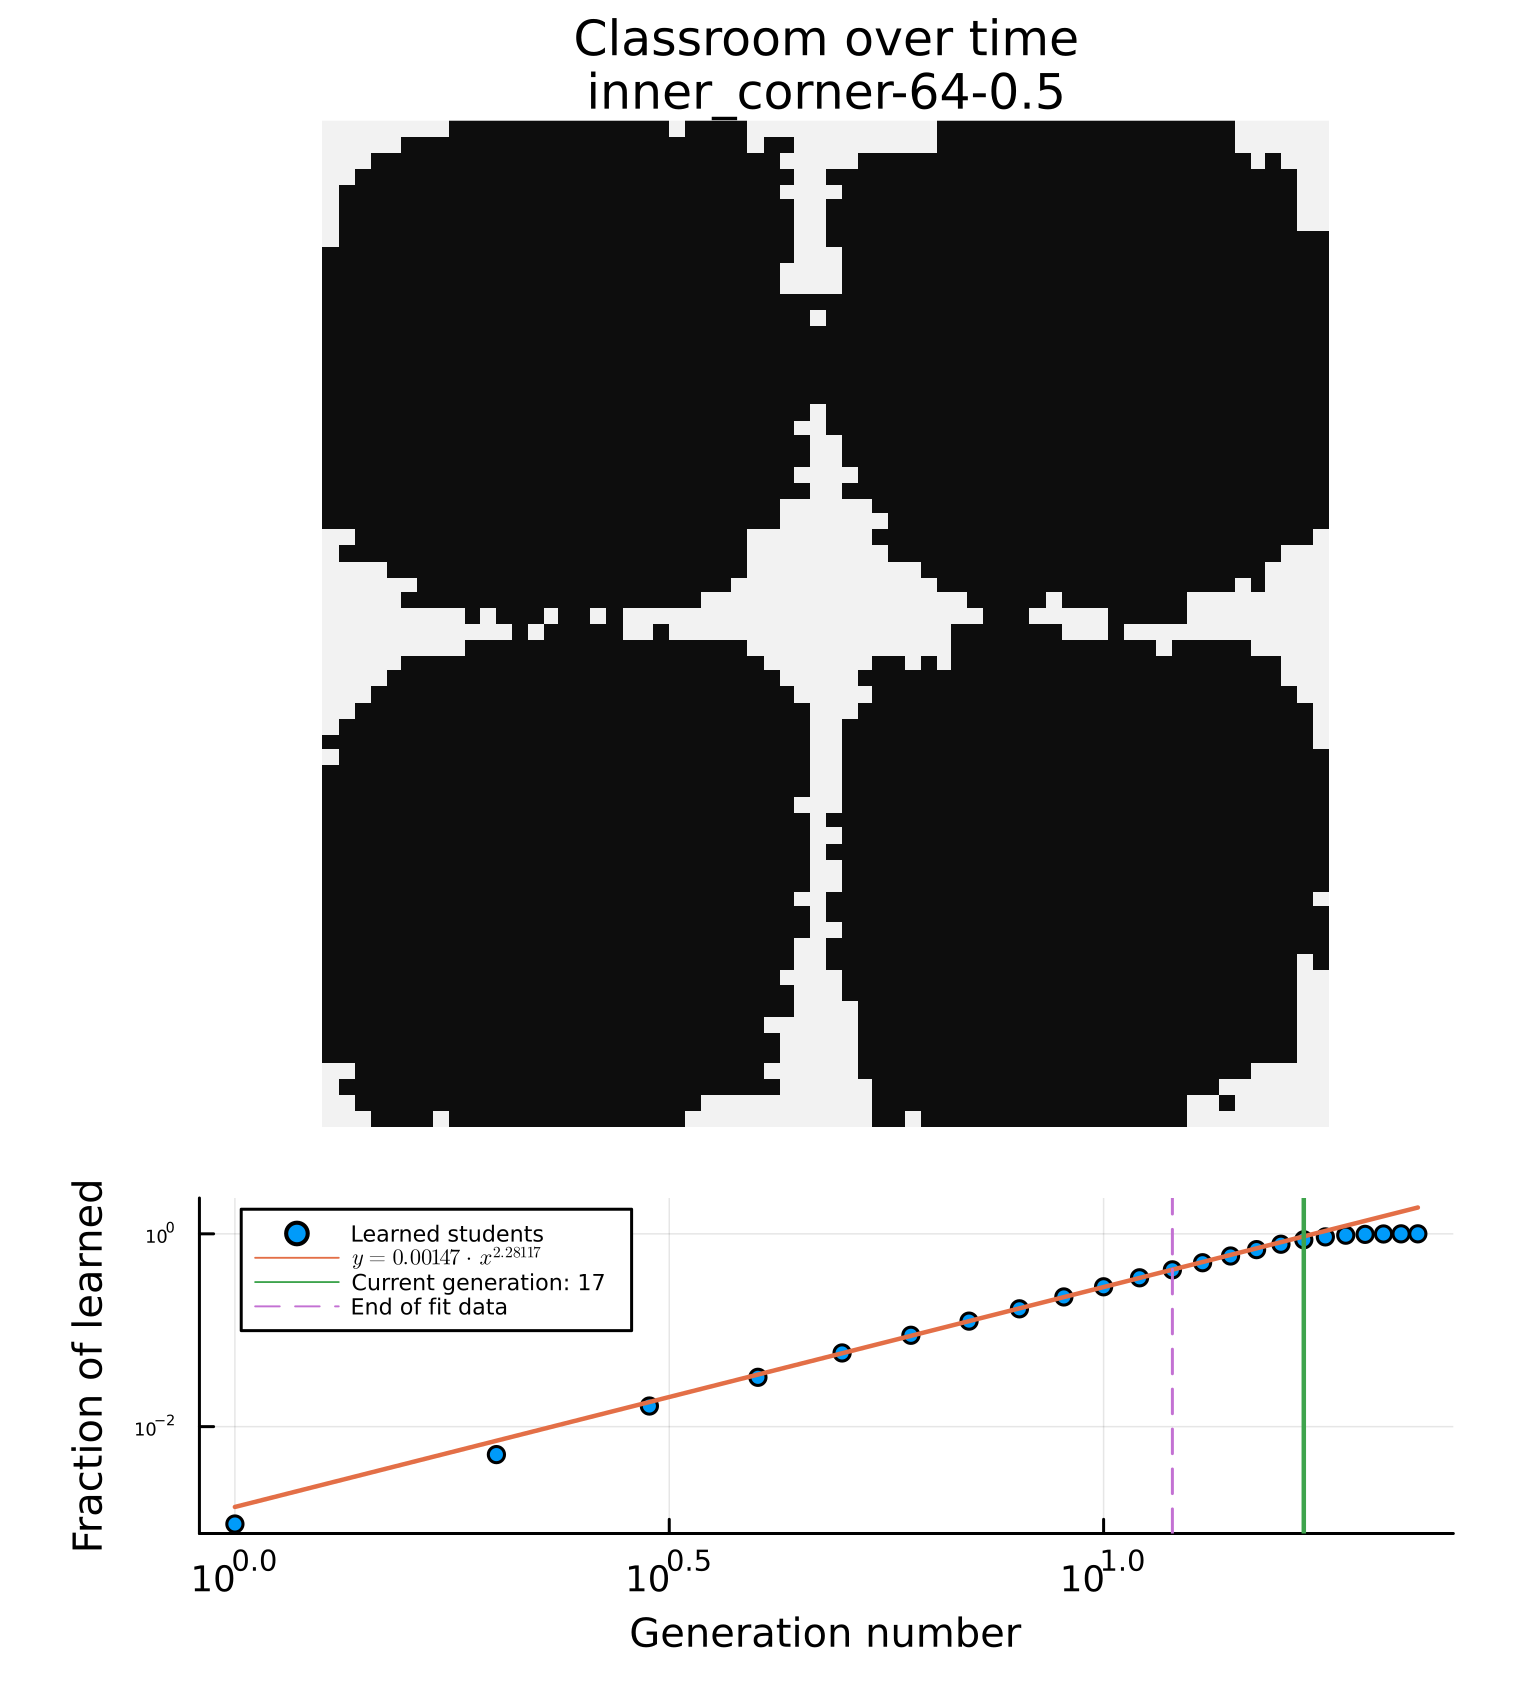
\includegraphics[width=0.45\textwidth]{figures/2D-BPCA-analysis/sample run - PI/2DBPCA-random-64-0.5-17.png}}
    \subfigure[$t=23$]{\label{fig:2DBPCA classroom 1}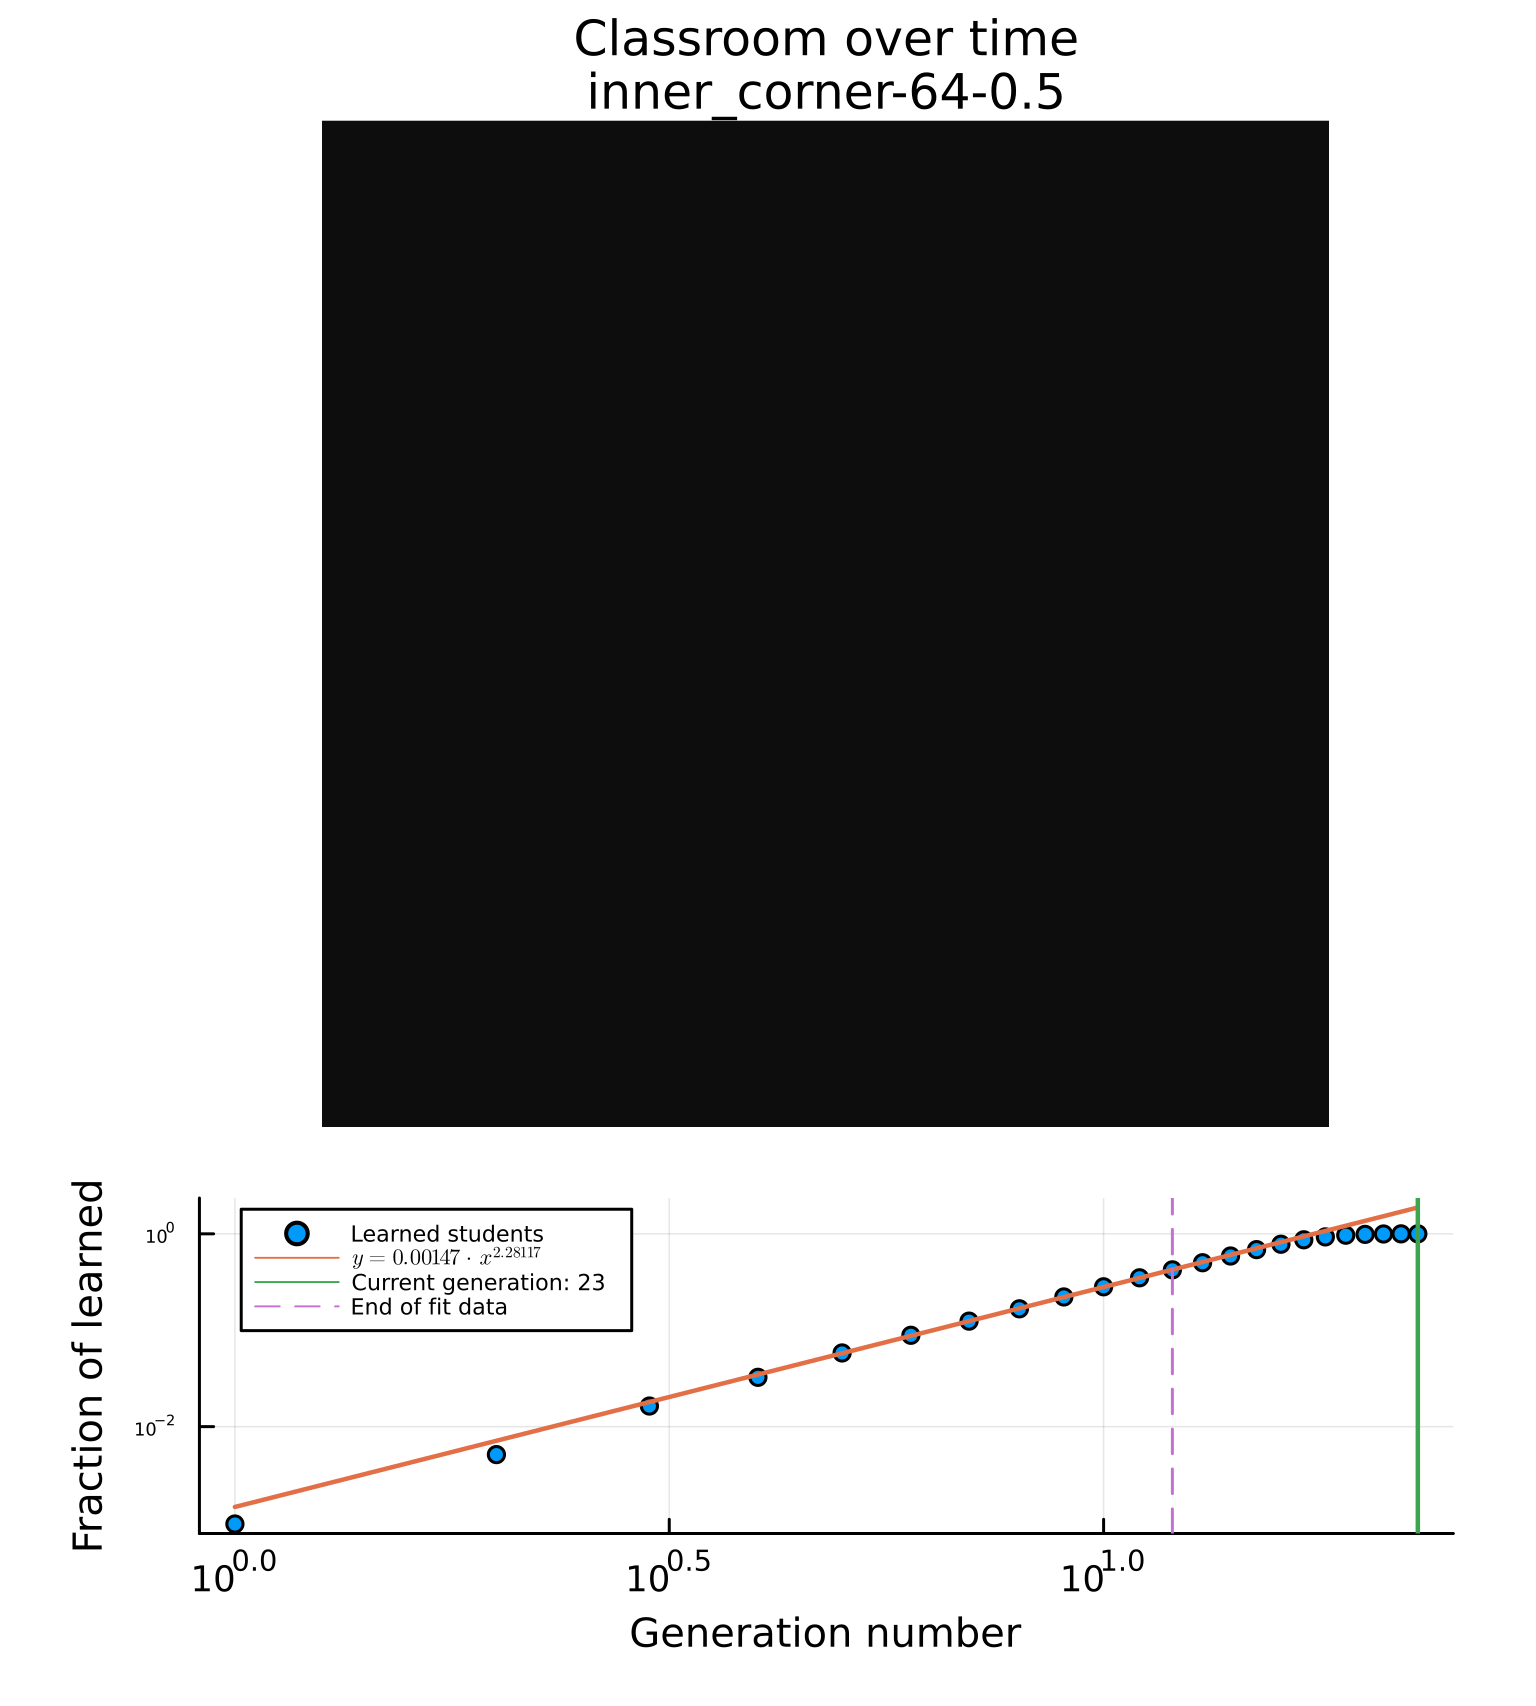
\includegraphics[width=0.45\textwidth]{figures/2D-BPCA-analysis/sample run - PI/2DBPCA-random-64-0.5-23.png}}
    \caption{Sample classroom evolution for $L=64$, $\lambda_0 = 1$, and $\rho_0 = 0.5$ with the inner corner SA. 
    Black squares represent learned students while white squares represent unlearned students. 
    The accompanying graphs show the fraction of learned students as a function of time. 
    The blue circle represents the data points while the orange line shows the power law fit. 
    The broken pink line shows the where we truncate the data for fitting the power law and the green line shows the current time step in the plot.}
    \label{fig:Sample classroom evolution}
 \end{figure}

\section{Results: Homogenous PI vs Traditional}
In this chapter, we only consider the case where all students have the same learning rate $\lambda_{i,j} = \lambda_0 = 1$ and an isotropic positional learning factor $\rho_{i,j} = \rho_0 \space ~\forall~ (\delta i \land \delta j),  \delta i, \delta j \in \lbrace -1,0,1 \rbrace $. 
From the simulations, we compared both the average number time steps $\langle t_{max} \rangle$ it takes for all the students in the classroom to learn and the average learning rate $\langle m \rangle$ across different configurations over 5 independent runs.
 The class learning rate $m$ for each trial was obtained by using a Levenberg-Marquardt algorithm to fit a power law ($y = ax^m$) to the fraction of learned students as a function of the generation number. 
 We only considered the first $50\%$ of the data for the PI model and the first $25\%$ of the data for the traditional model. 
This truncation was done so that we only fit the part of the data before the finite size effect starts to affect the simulation.

\subsection{Time to learn $t_{max}$ vs positional learning factor $\rho_0$} \label{subsec: 2DBPCA tmax vs rho}

The data in Figure \ref{fig:2DBPCA tmax vs rho} shows that the time to learn $t_{max}$ decreases with increasing positional learning factor $\rho_0$ for all classroom sizes for both traditional models and PI models. 
Among PI models, the inner corner configuration has the lowest $t_{max}$ for all classroom sizes. 
The outer corner and center SAs performed similarly, while the random SA has the highest $t_{max}$. 
The traditional model performs situationally better than even the inner corner PI model, something we will investigate in Section \ref{subsec: 2DBPCA tmax vs N}.

\begin{figure}[htbp!]
    \centering
    \subfigure[$L=32$]{\label{fig:2DBPCA tmax vs rho 32}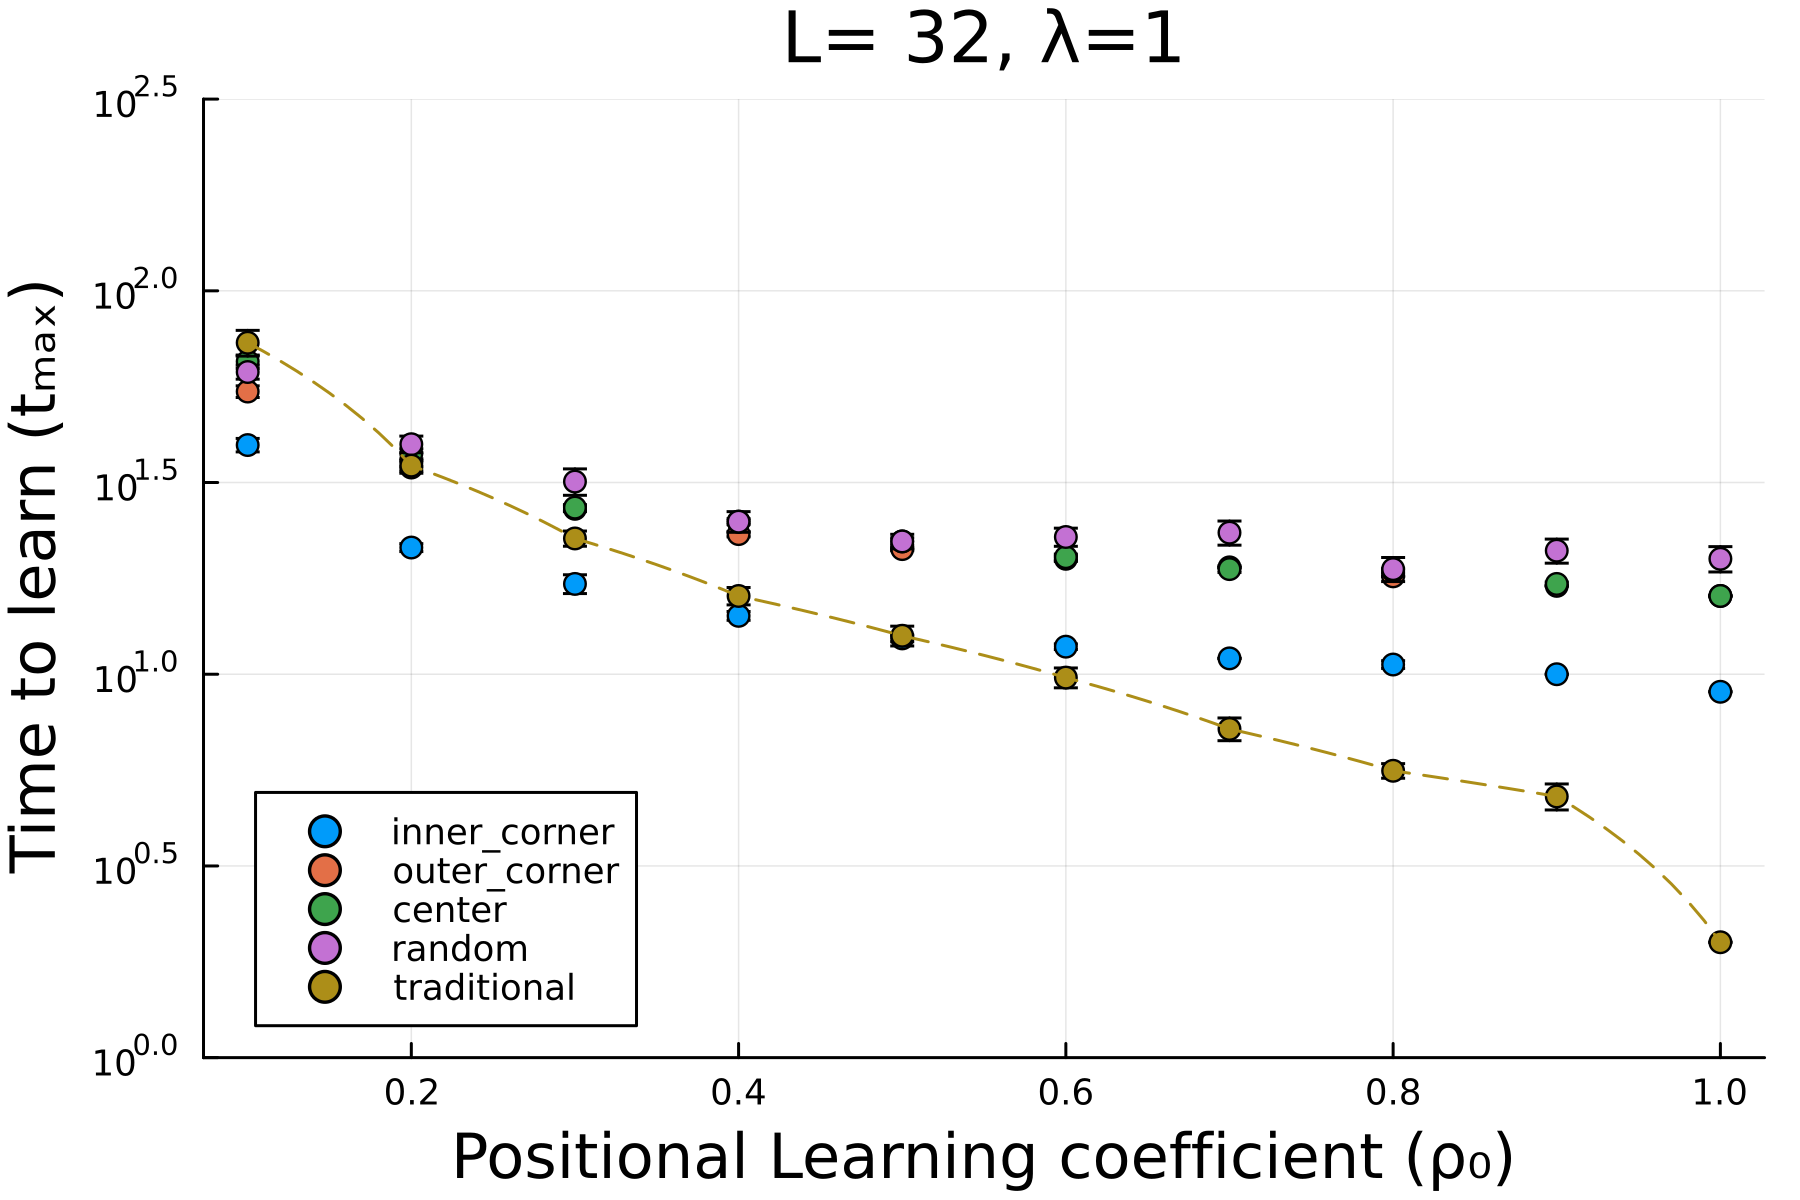
\includegraphics[width=0.45\textwidth]{figures/2D-BPCA-analysis/t-32.png}}
    \subfigure[$L=48$]{\label{fig:2DBPCA tmax vs rho 48}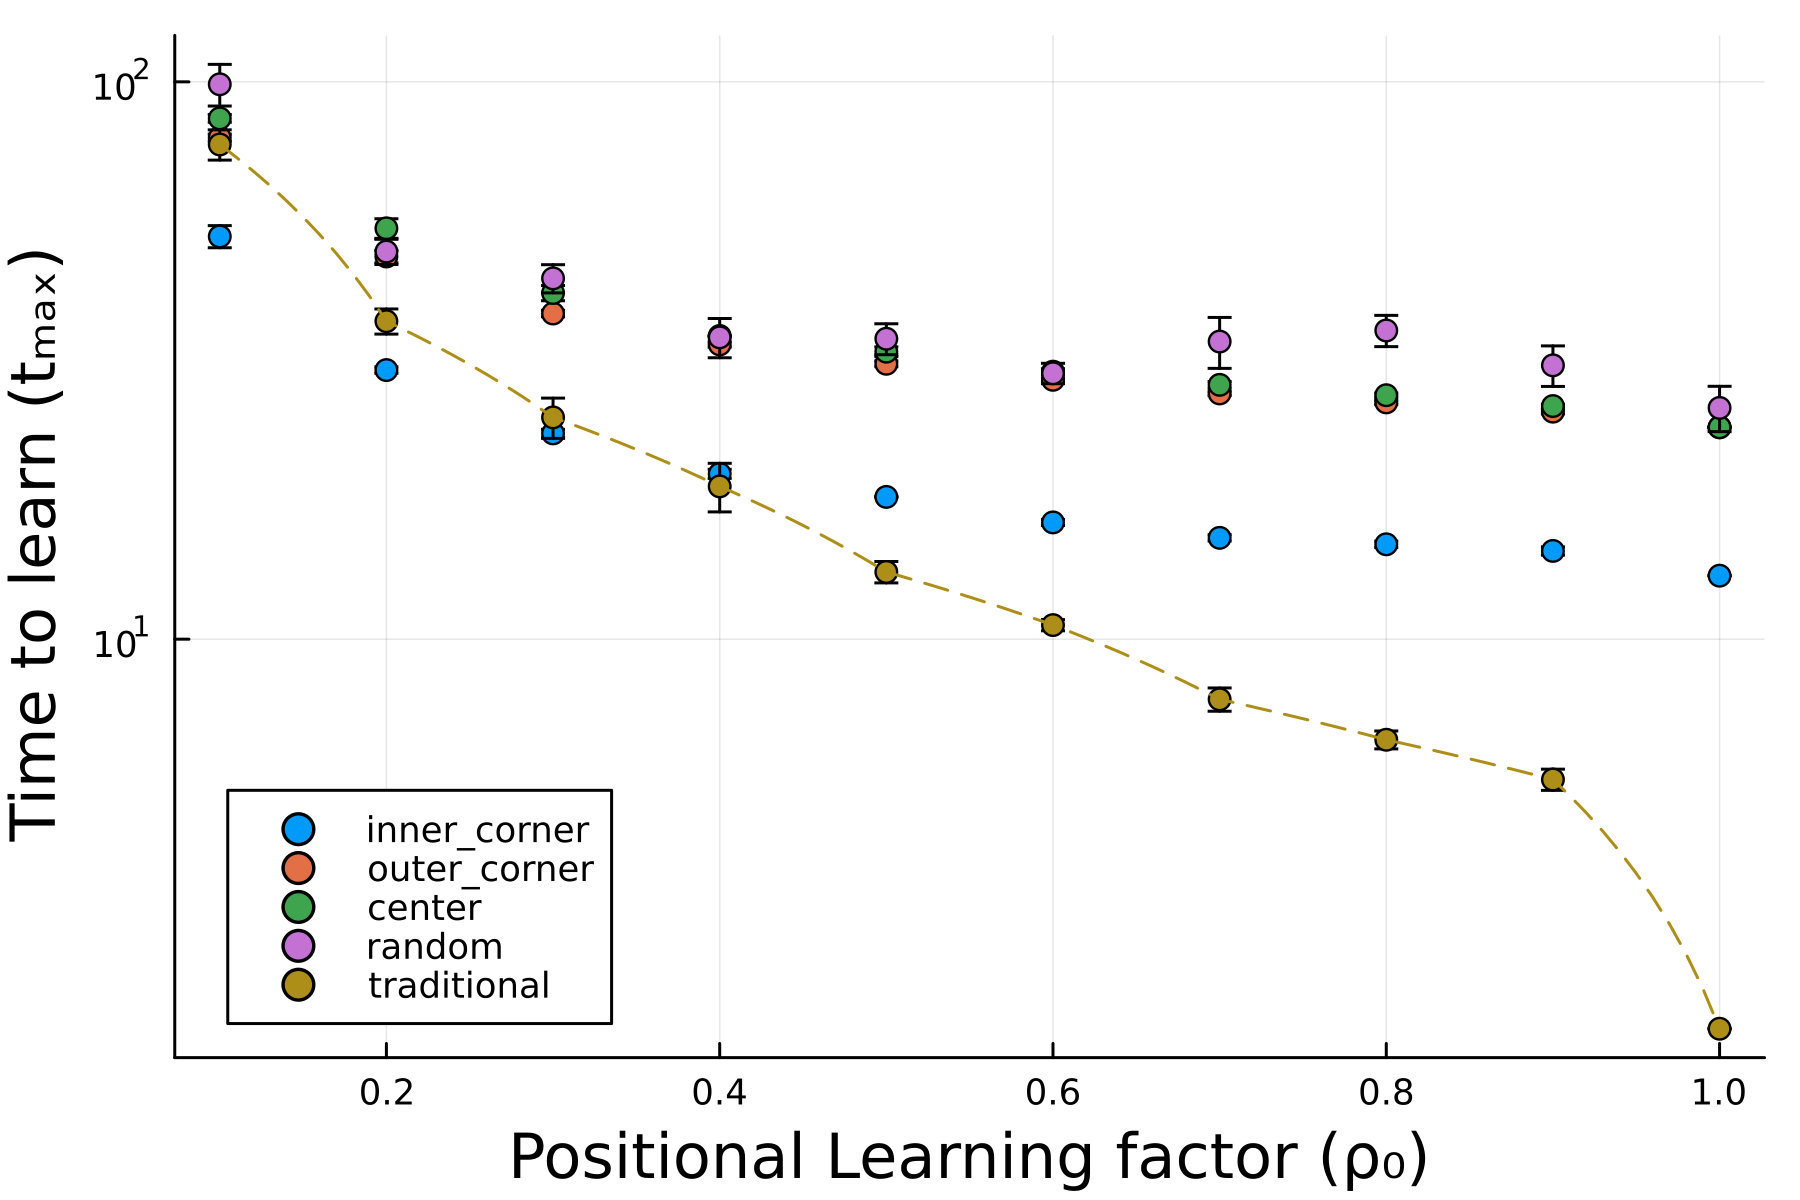
\includegraphics[width=0.45\textwidth]{figures/2D-BPCA-analysis/t-48.png}}
    \subfigure[$L=64$]{\label{fig:2DBPCA tmax vs rho 64}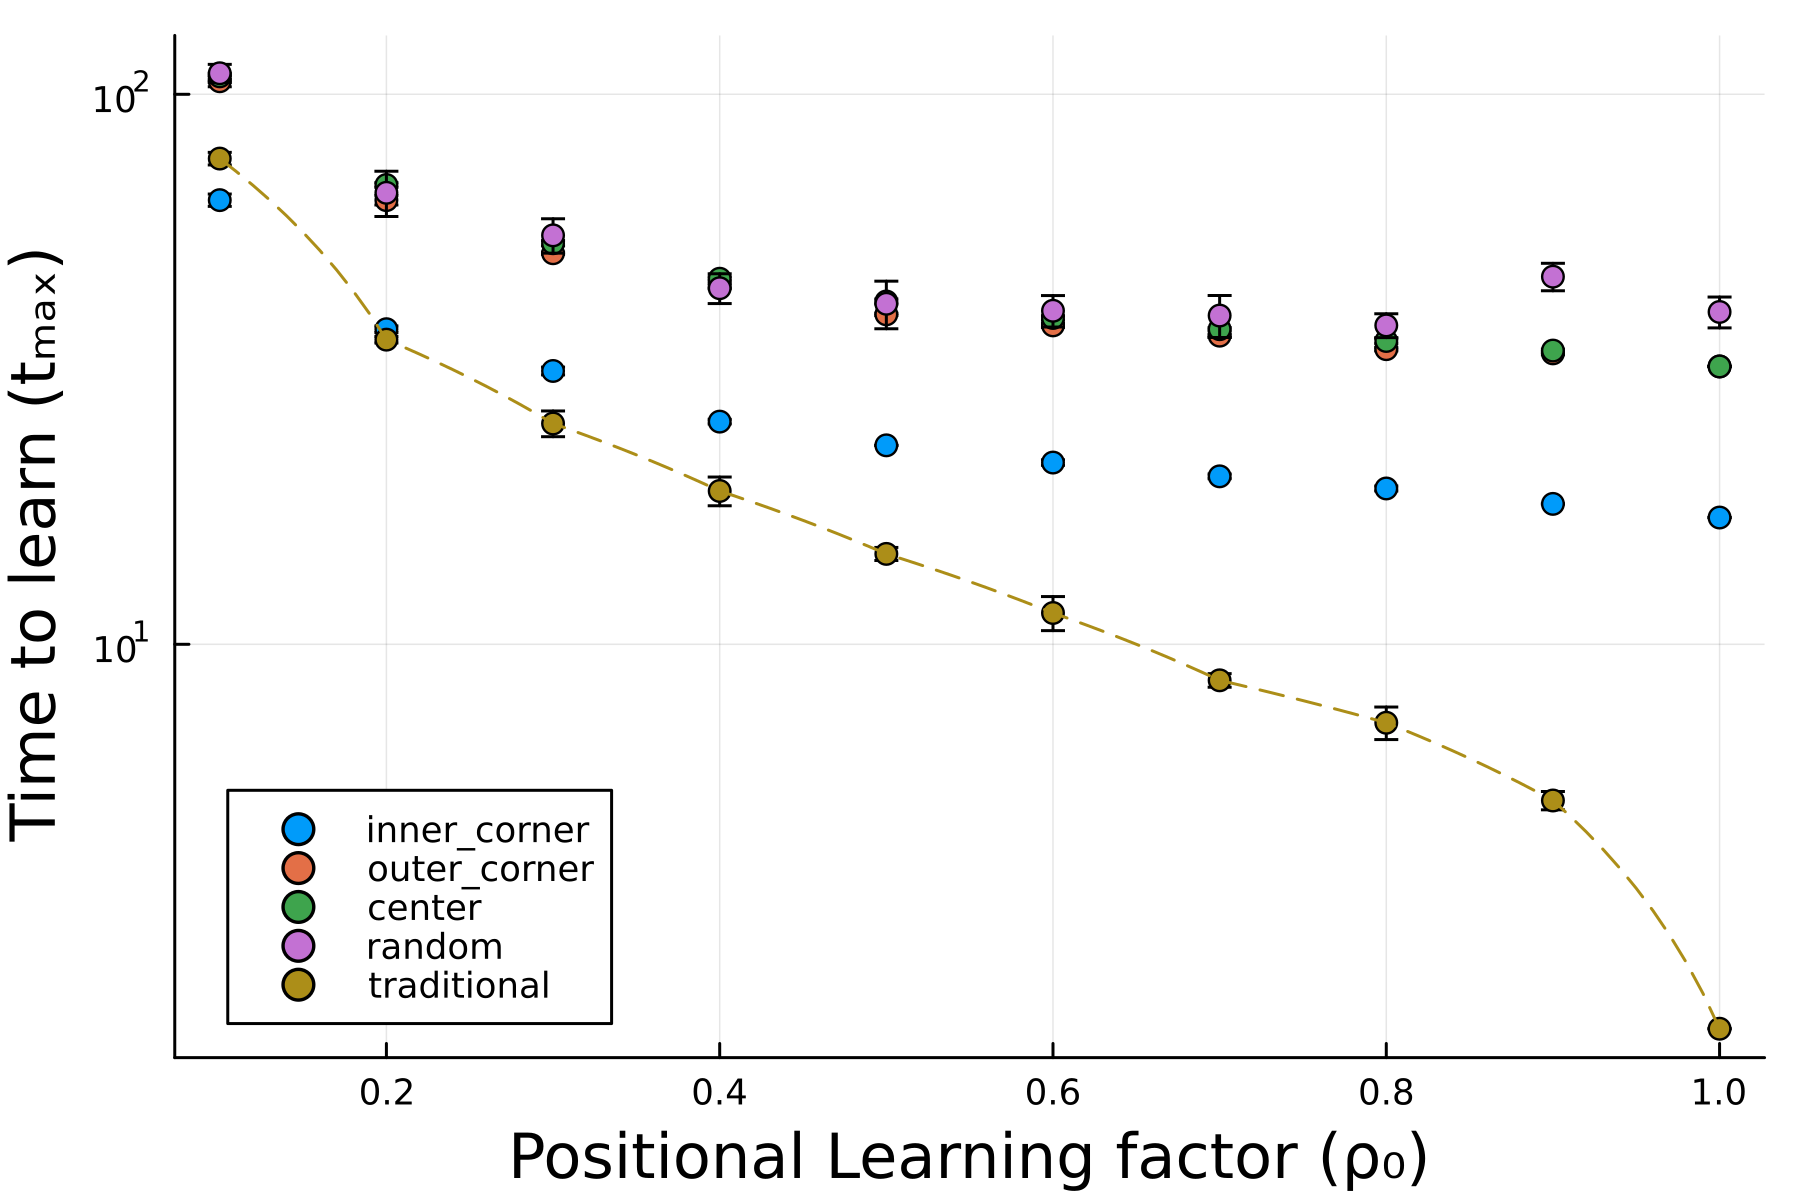
\includegraphics[width=0.45\textwidth]{figures/2D-BPCA-analysis/t-64.png}}
    \subfigure[$L=96$]{\label{fig:2DBPCA tmax vs rho 96}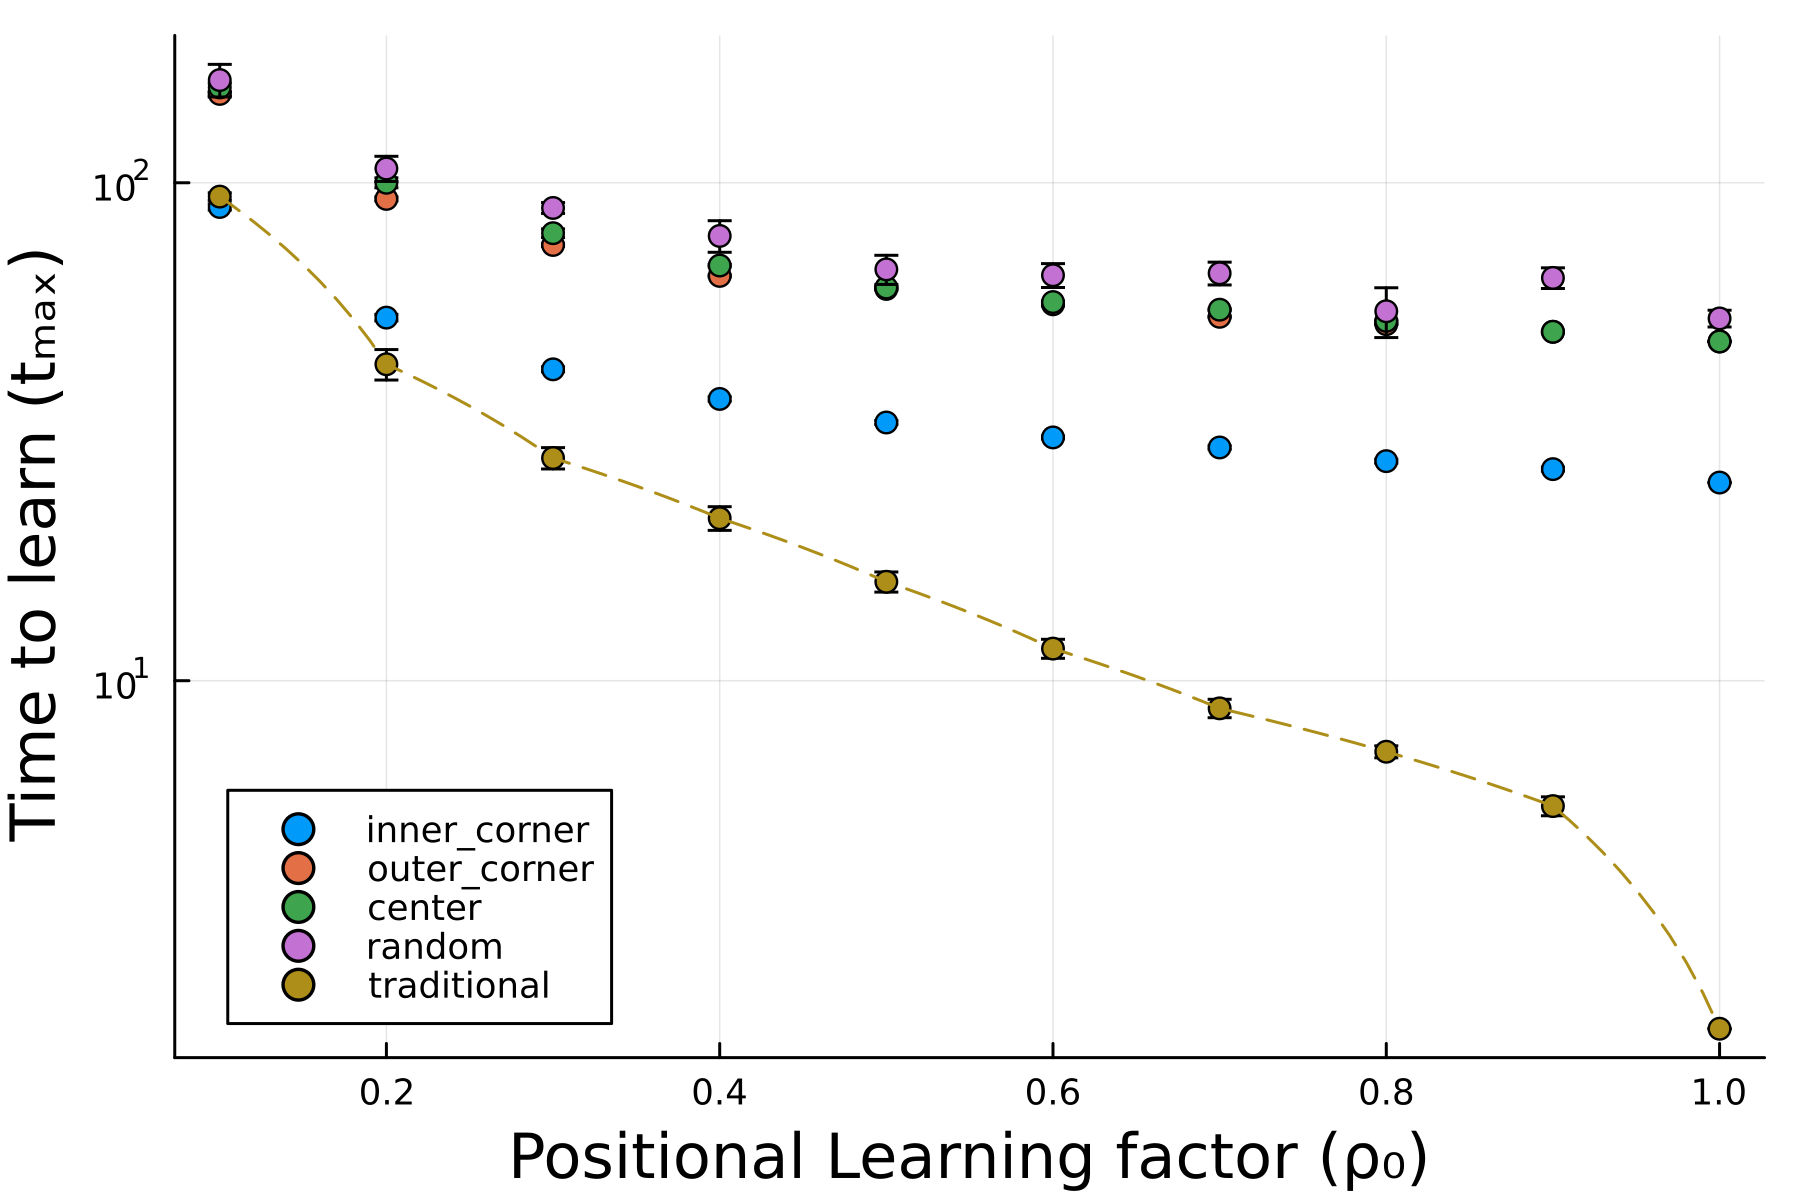
\includegraphics[width=0.45\textwidth]{figures/2D-BPCA-analysis/t-96.png}}
    \subfigure[$L=128$]{\label{fig:2DBPCA tmax vs rho 128}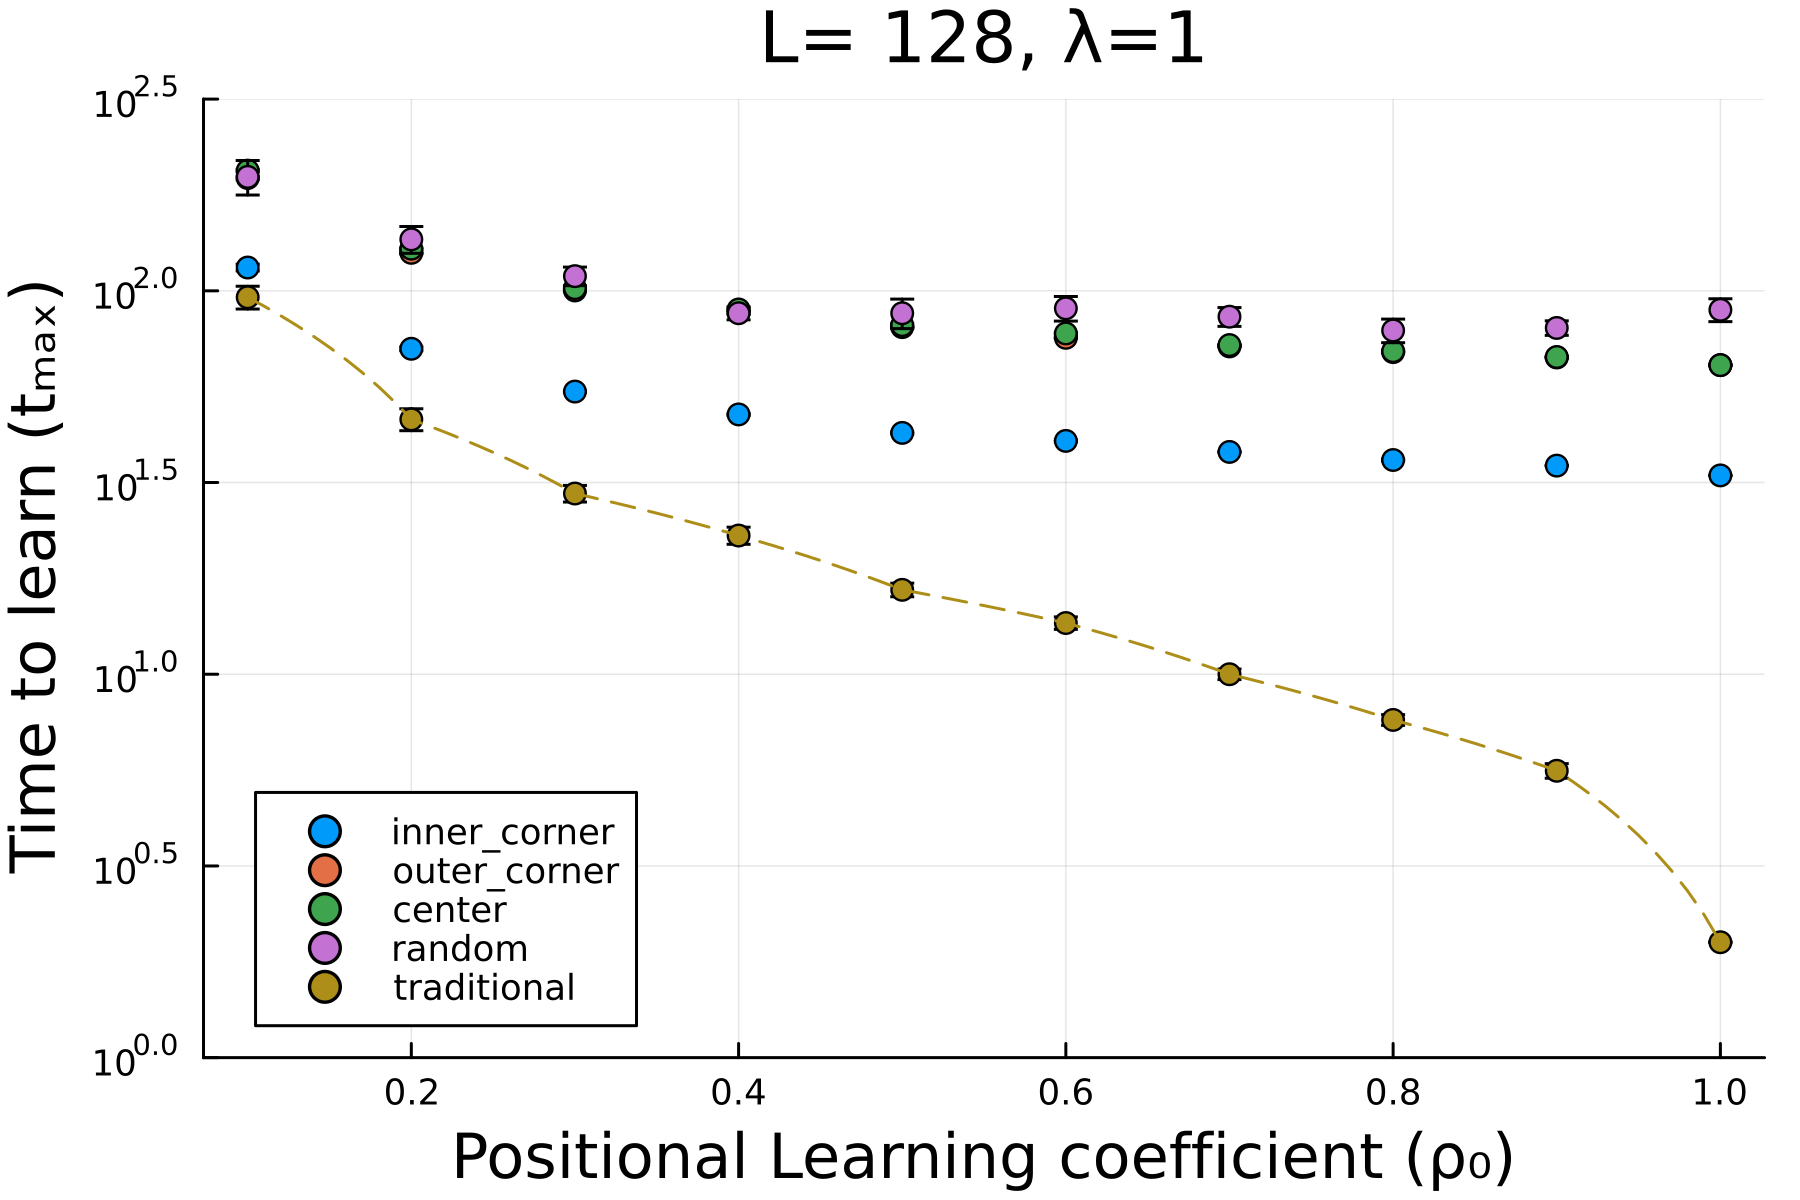
\includegraphics[width=0.45\textwidth]{figures/2D-BPCA-analysis/t-128.png}}
    \caption{Time to learn $t_{max}$ as a function of positional learning factor $\rho_0$ for different classroom sizes $L \in \lbrace 32,48,64,96,128 \rbrace$. 
    Lower time to learn $t_{max}$ indicate better performance.}
    \label{fig:2DBPCA tmax vs rho}
\end{figure}

\newpage

\subsection{Class learning rate $m$ vs positional learning factor $\rho_0$}

The data in Figure \ref{fig:2DBPCA m vs rho} shows that the class learning rate $m$ does not generally change for different positional learning factors $\rho_0$ when comparing against similar SAs for the PI model. 
The traditional model, however, shows a increase in class learning rate $m$ with increasing $\rho_0$ for all classroom sizes. 
Similar to the findings in section \ref{subsec: 2DBPCA tmax vs rho}, the inner corner configuration has the highest learning rate $m$ for all classroom sizes. 
The outer corner and center SAs performed similarly, while the random SA has the lowest class learning rate $m$. We still find that the traditional model performs situationally better than even the inner corner PI model. 

The sudden decrease in class learning rate $m$ for the traditional model at $\rho_0 = 1.0$ is due to the improper truncation and fitting of the data. 
In the traditional model where $\rho_0 = 1.0$, all the students will transition from unlearned to learned in one time step, so fitting the power law to the first 25\% of the data would yield a class learning rate $m$ that does not represent the results of the simulations well.

We notice that these results differ slightly from the ones presented in section \ref{subsec: 2DBPCA tmax vs rho}. 
The results in this section show that the traditional model performs better than the PI model in terms of class learning rate $m$ for all classroom sizes at low $\rho_0$. 
This is in contrast to the results in section \ref{subsec: 2DBPCA tmax vs rho} where the PI model performed better only in small classrooms with low positional learning factor $\rho_0$. 
This discrepancy is likely due to the different metrics used to evaluate the performance of the models. The class learning rate $m$ is a measure of how quickly the students learn, while the time to learn $t_{max}$ is a measure of how long it takes for all the students to learn. 
In cases where the classroom is large and positional learning factor $\rho_0$ is small, the traditional model is able to teach all the students in a shorter amount of time despite the PI model being able to teach the students more effectively. 
\textit{This could be what other researches find when they claim that PI is a more effective method without accounting for the classroom room size or the students' learning rates. citation needed}

\begin{figure}[htbp!]
    \centering
    \subfigure[$L=32$]{\label{fig:2DBPCA m vs rho 32}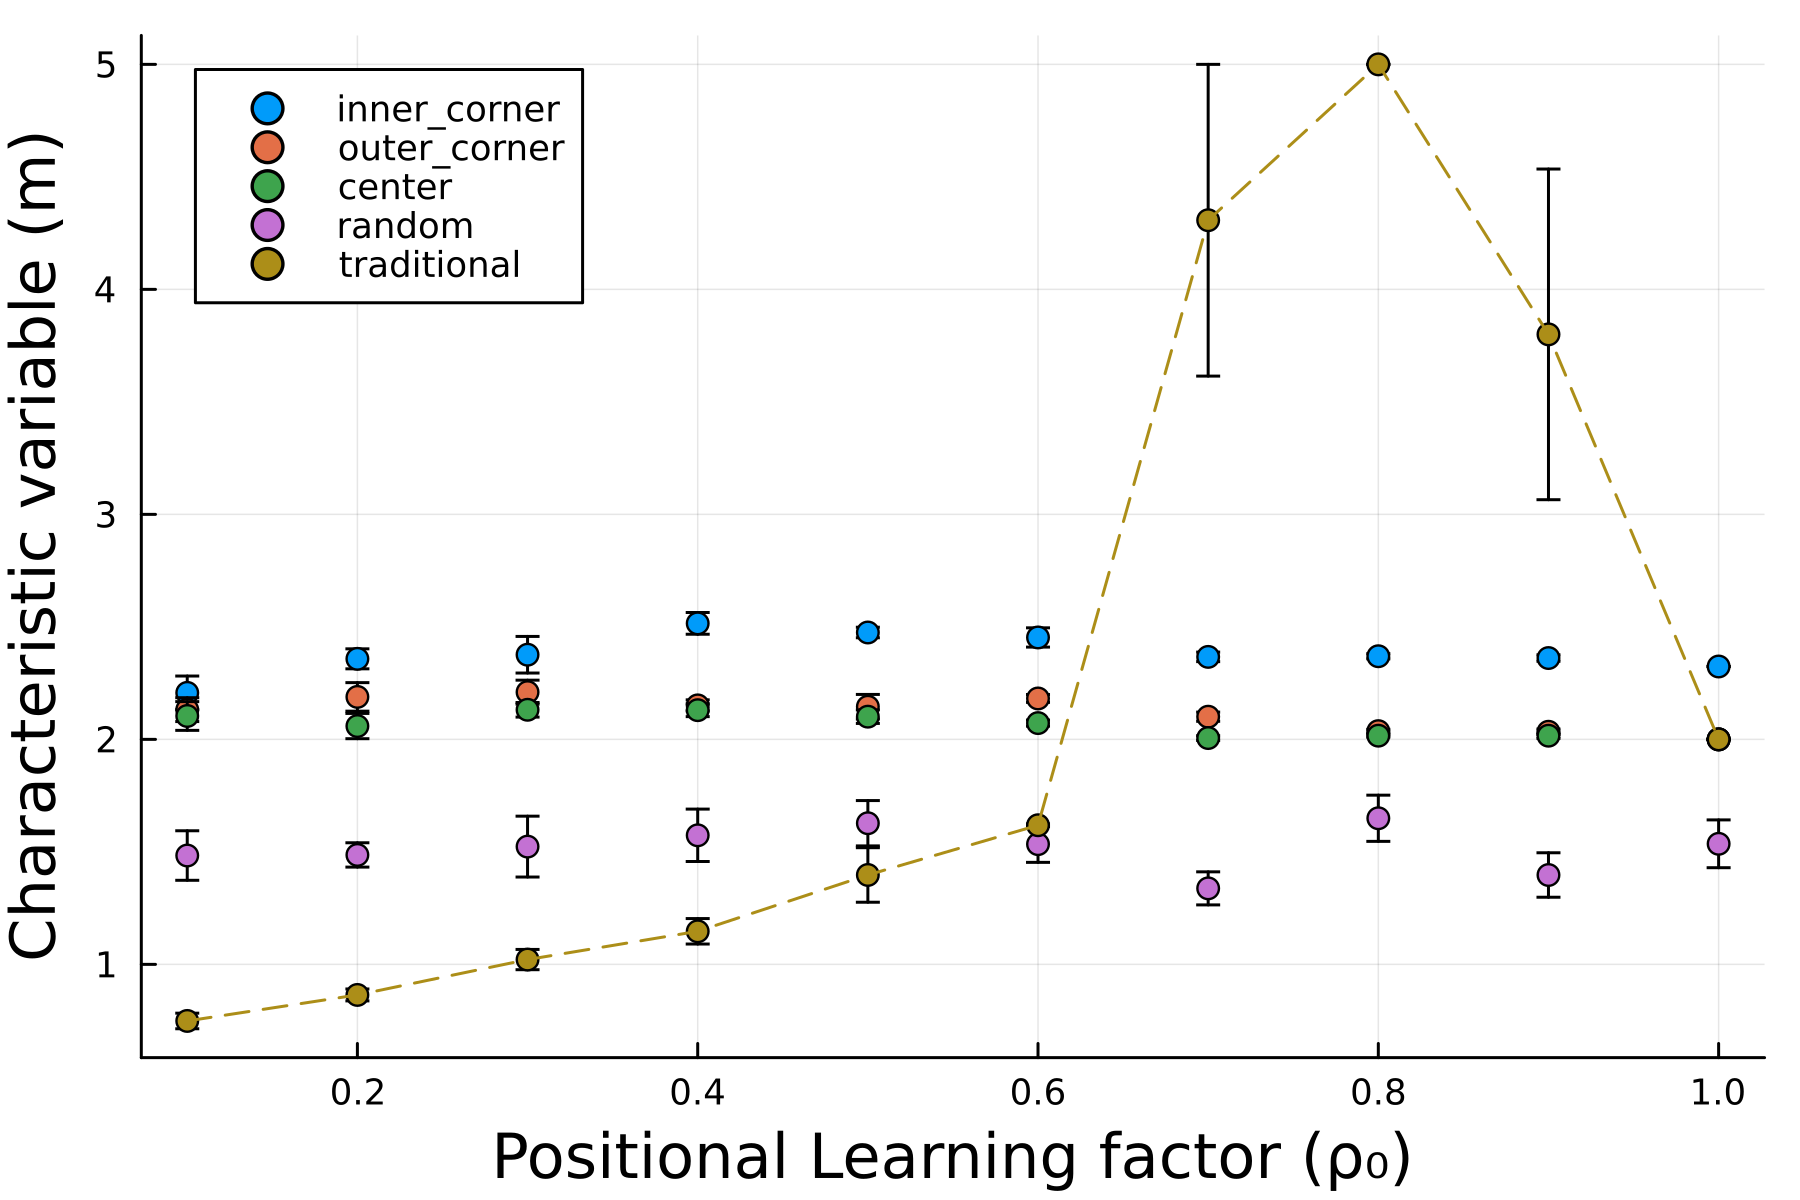
\includegraphics[width=0.45\textwidth]{figures/2D-BPCA-analysis/m-32.png}}
    \subfigure[$L=48$]{\label{fig:2DBPCA m vs rho 48}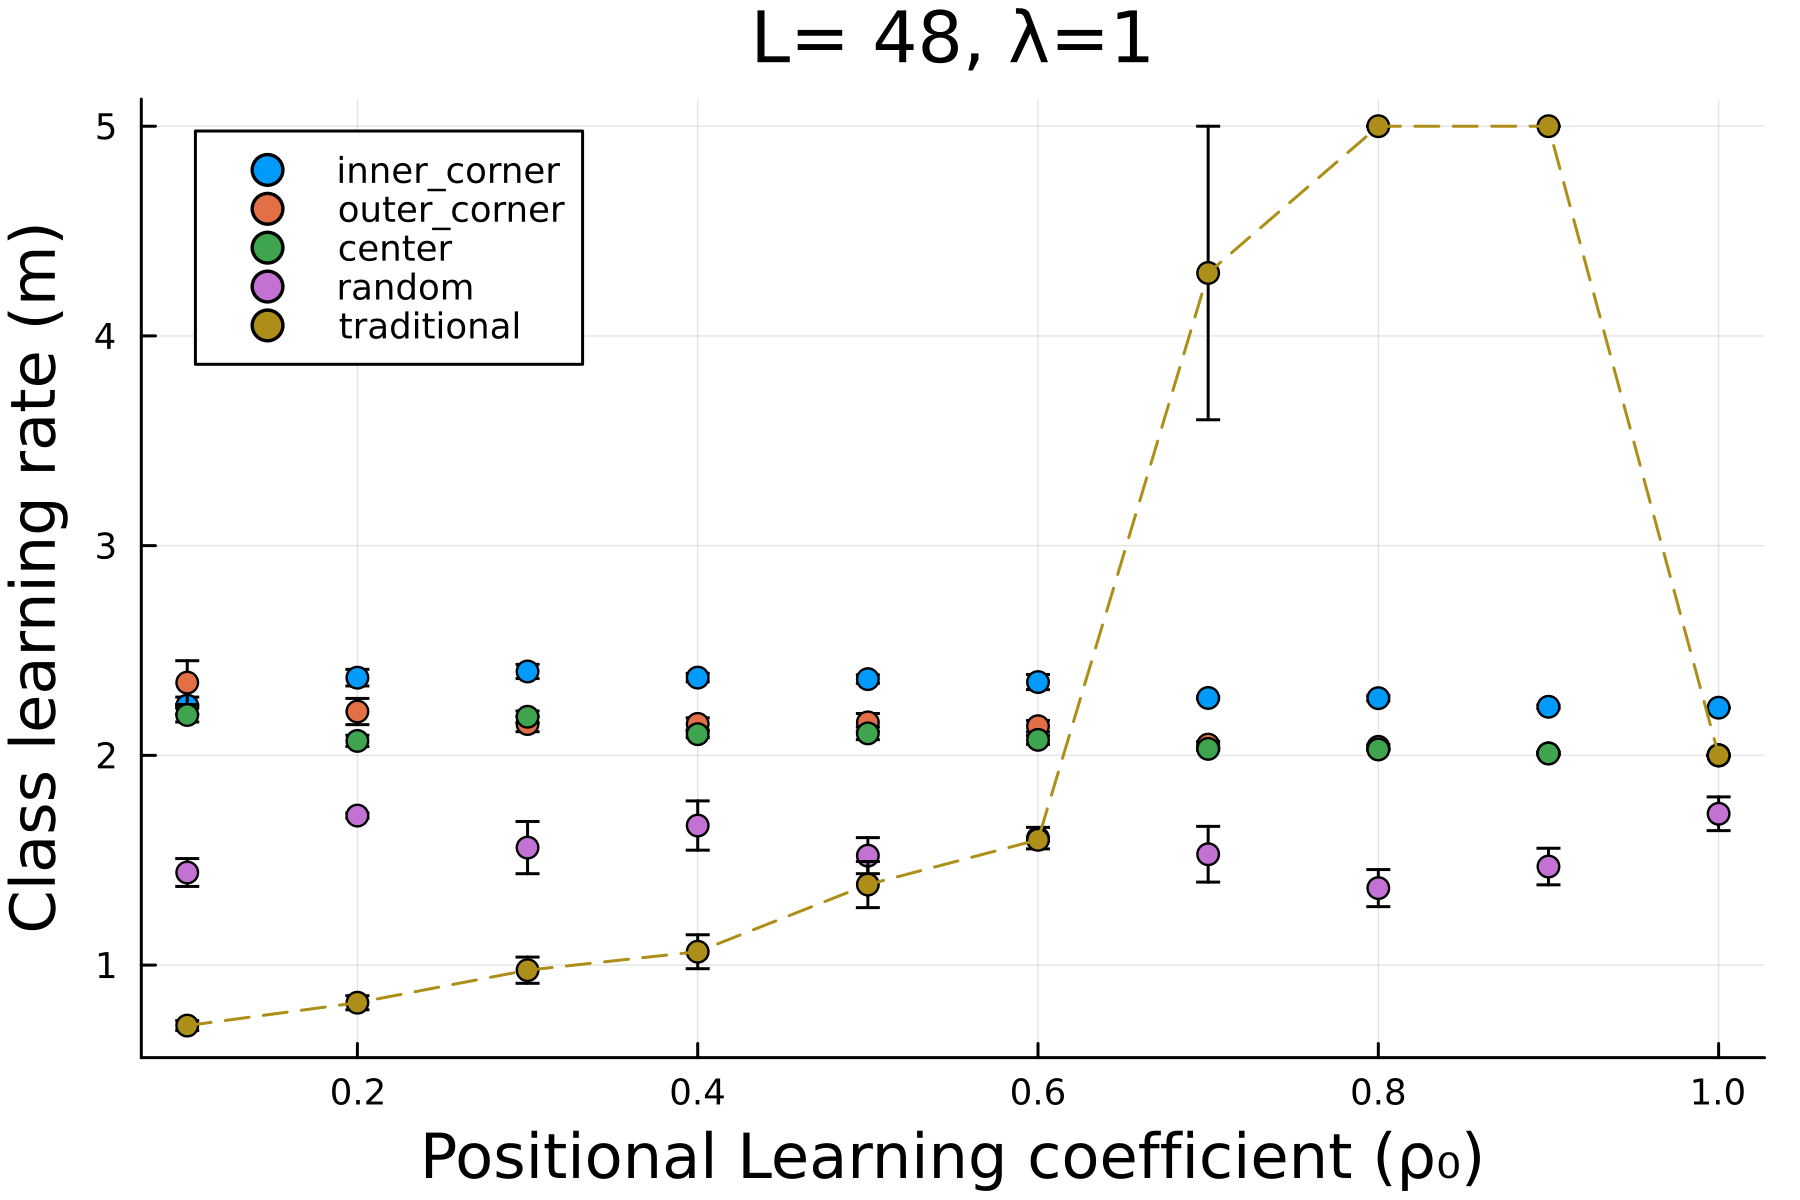
\includegraphics[width=0.45\textwidth]{figures/2D-BPCA-analysis/m-48.png}}
    \subfigure[$L=64$]{\label{fig:2DBPCA m vs rho 64}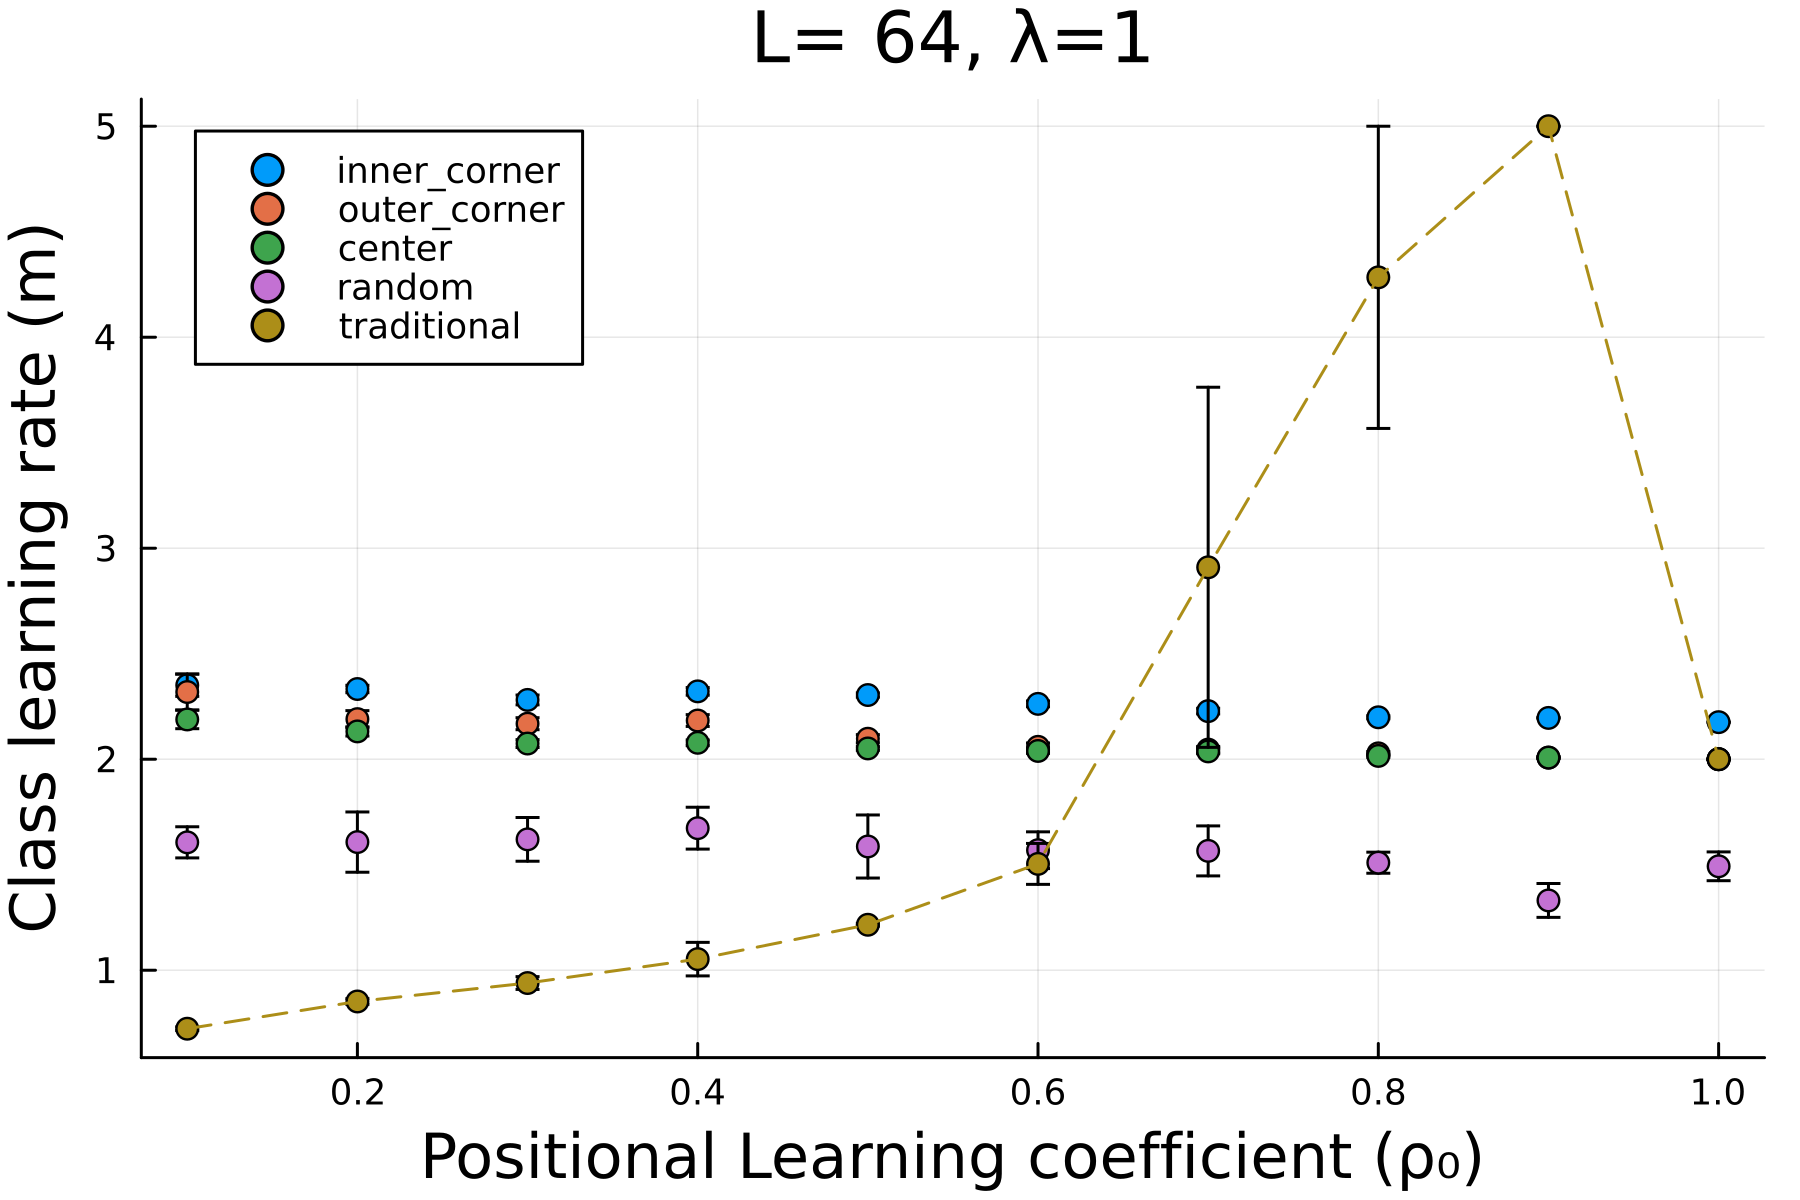
\includegraphics[width=0.45\textwidth]{figures/2D-BPCA-analysis/m-64.png}}
    \subfigure[$L=96$]{\label{fig:2DBPCA m vs rho 96}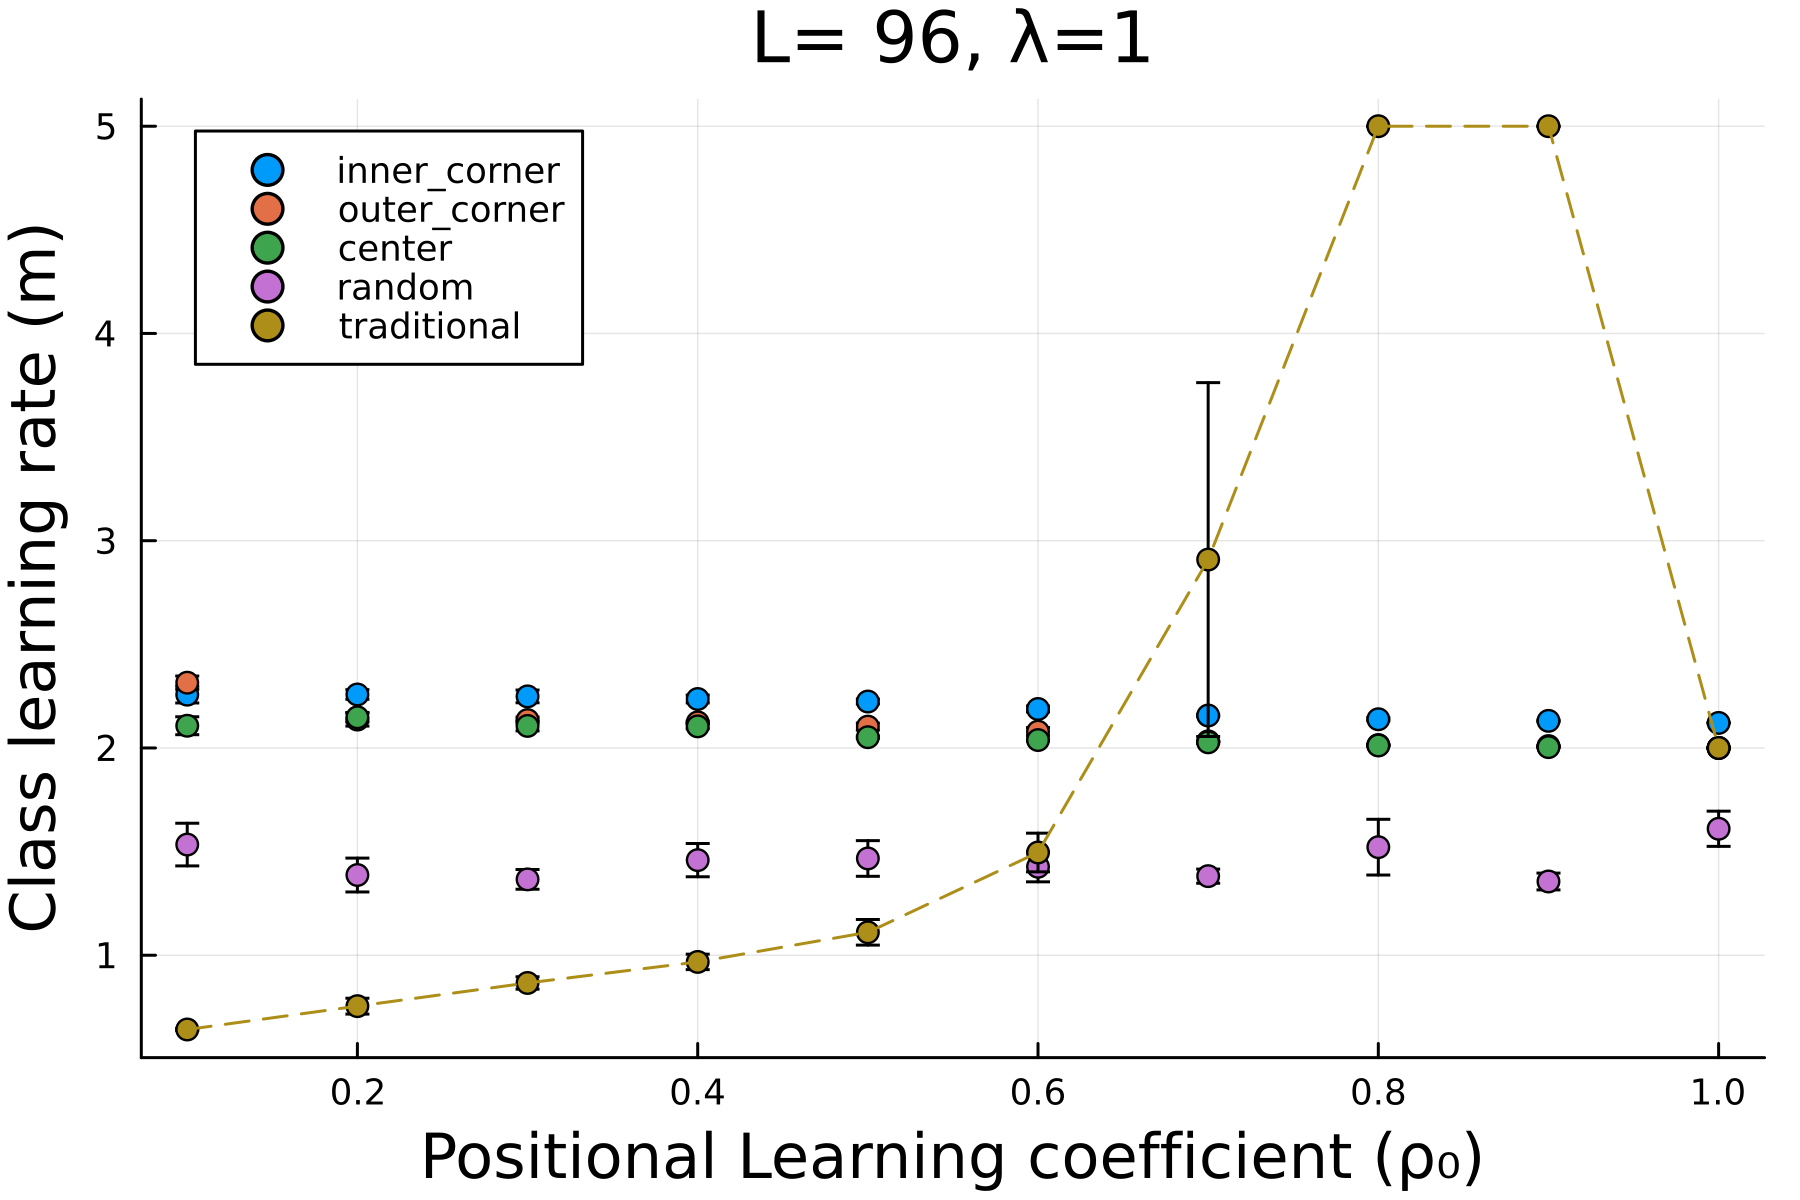
\includegraphics[width=0.45\textwidth]{figures/2D-BPCA-analysis/m-96.png}}
    \subfigure[$L=128$]{\label{fig:2DBPCA m vs rho 128}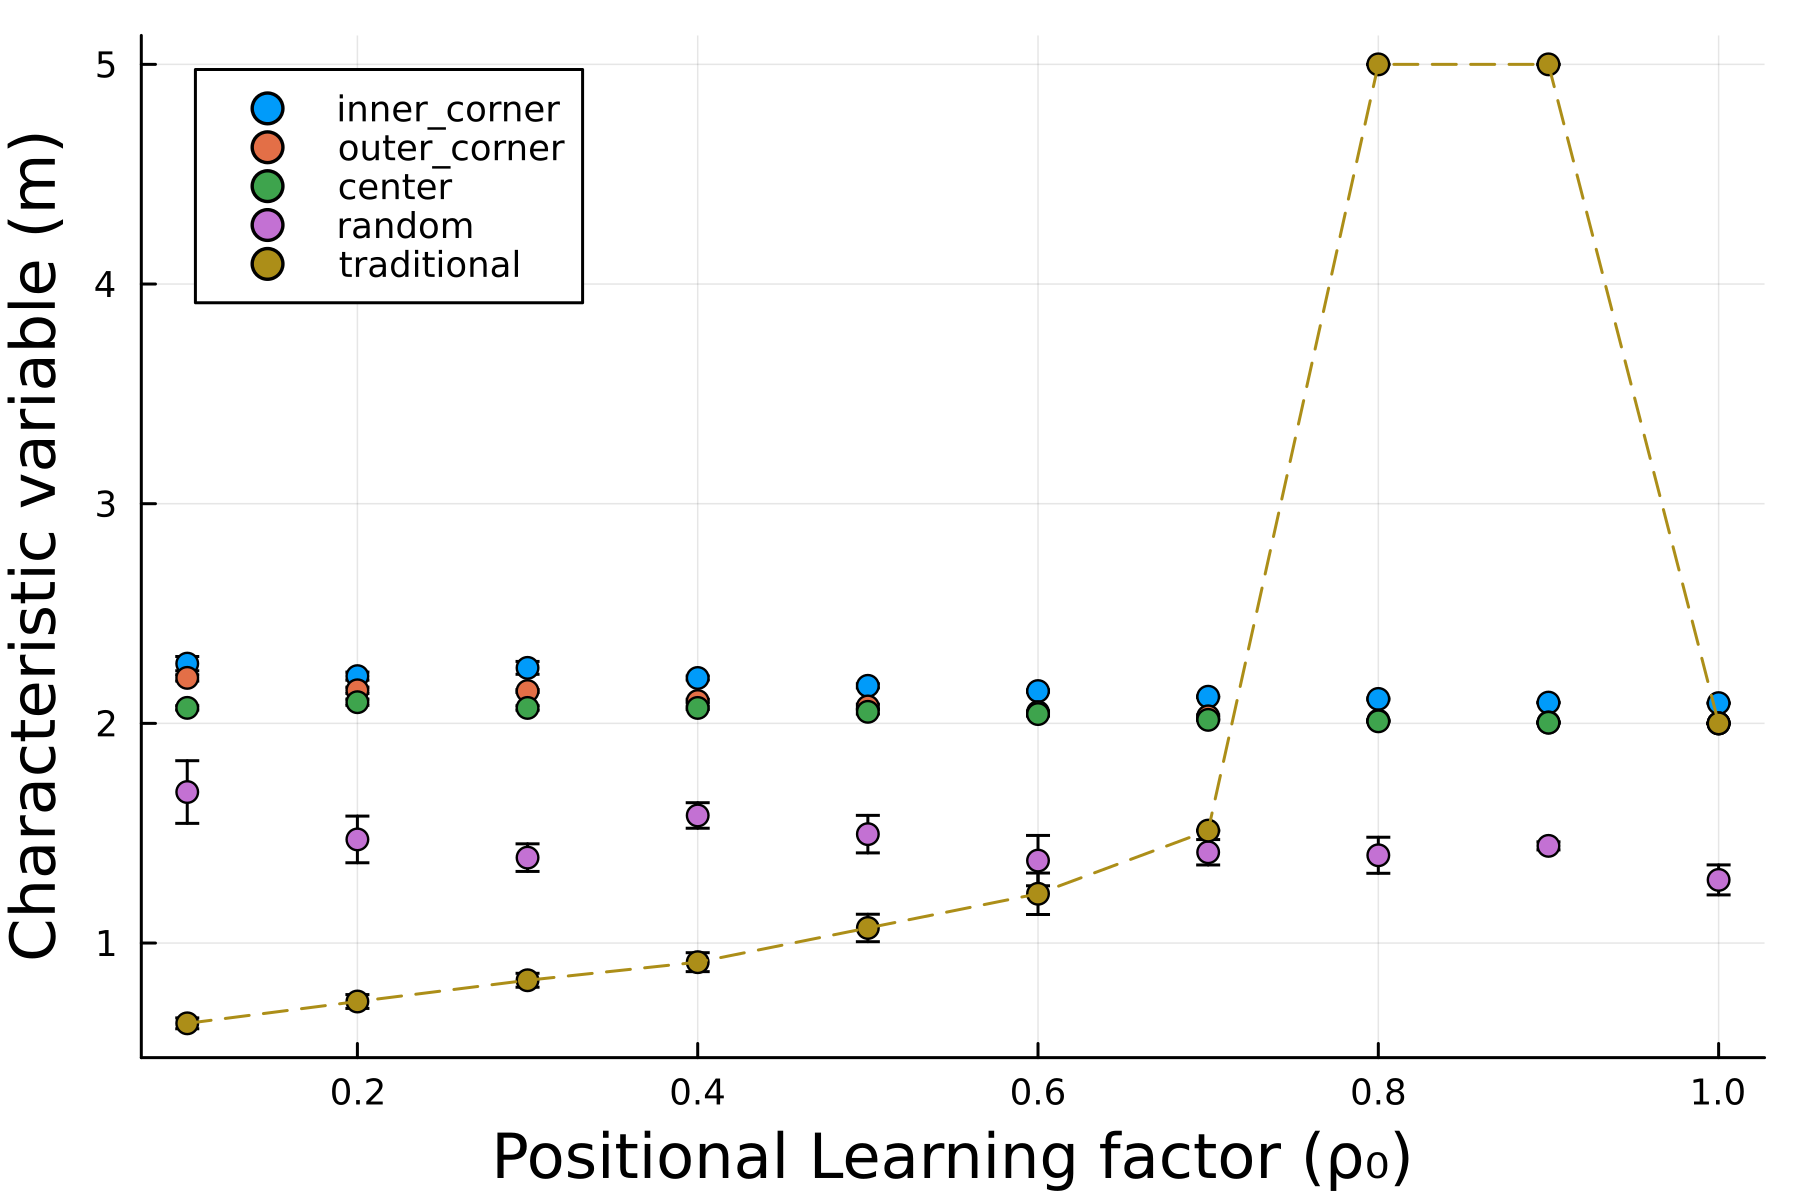
\includegraphics[width=0.45\textwidth]{figures/2D-BPCA-analysis/m-128.png}}
    \caption{Class learning rate $m$ as a function of positional learning factor $\rho_0$ for different classroom sizes $L \in \lbrace 32,48,64,96,128 \rbrace$. 
    Higher class learning rate $m$ values indicate better performance.}
    \label{fig:2DBPCA m vs rho}
\end{figure}

\newpage

\subsection{Time to learn $t_{max}$ vs class size $N$} \label{subsec: 2DBPCA tmax vs N}
\begin{figure}[h!]
    \centering
    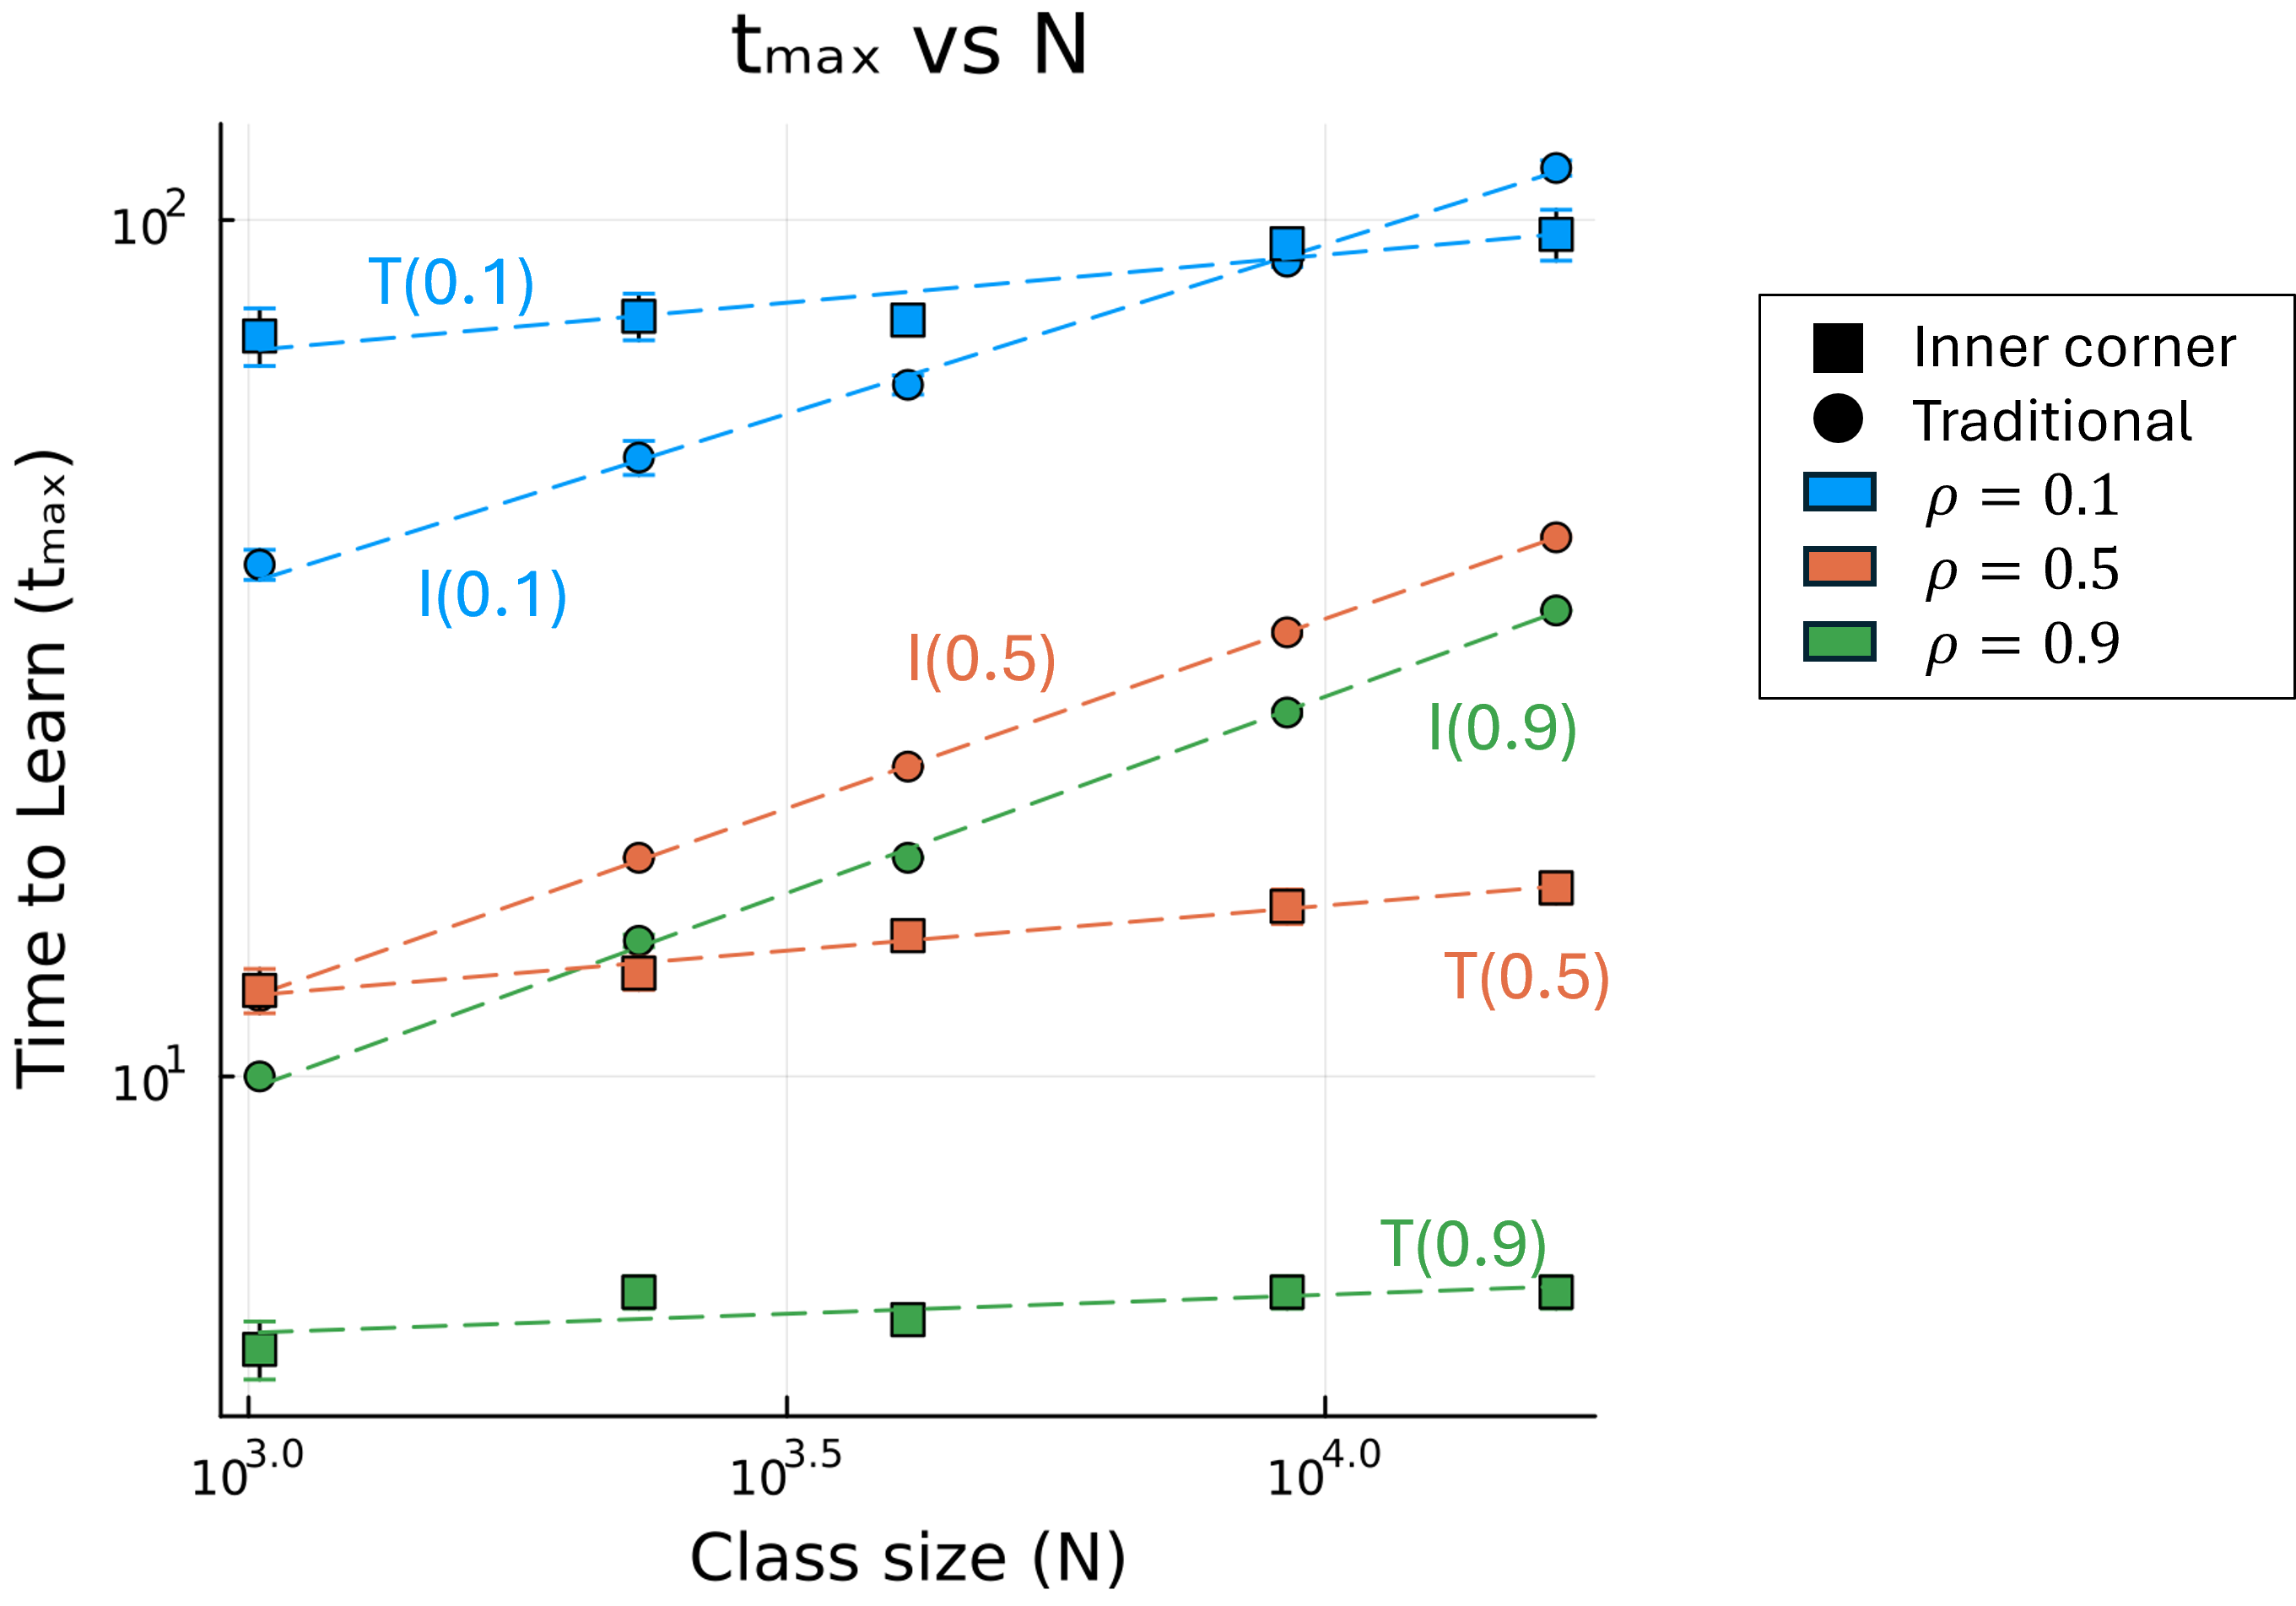
\includegraphics[width=0.8\textwidth]{figures/2D-BPCA-analysis/N_vs_tmax-traditional-inner_corner.png}
    \caption[Class size dependence of time to learn in homogenous models]{Time to learn $t_{max}$ as a function of class size $N$ for PI and traditional models. 
    Circles and squares denote data points for the inner corner PI configuration and traditional learning model, respectively. 
    The dash lines are the corresponding power law fit of the form $t_{max}=a \cdot N^b$ using $\rho \in \lbrace 0.1, 0.5, 0.9 \rbrace$. 
    The fitted parameters are shown in the table with an average of $\langle b \rangle = 0.4532 \pm 0.019$ for the inner corner and $\langle b \rangle = 0.087\pm0.021$ for the traditional model.}
    \label{fig:Traditional vs PI tmax vs N}
\end{figure}

\begin{table}[htbp!]
  \centering
  
  \begin{tabular}{|c|cc|cc|}
    \hline
    & \multicolumn{2}{c|}{\textbf{Inner corner}}       & \multicolumn{2}{c|}{\textbf{Traditional}}        \\ \cline{2-5} 
    & \multicolumn{1}{c|}{\textbf{$a$}} & \textbf{$b$} & \multicolumn{1}{c|}{\textbf{$a$}} & \textbf{$b$} \\ \hline
    \textbf{$\lambda=0.1$} & \multicolumn{1}{c|}{2.4515}       & 0.3955       & \multicolumn{1}{c|}{32.4884}      & 0.1119       \\ \hline
    \textbf{$\lambda=0.5$} & \multicolumn{1}{c|}{0.5795}       & 0.4428       & \multicolumn{1}{c|}{6.0079}       & 0.1052       \\ \hline
    \textbf{$\lambda=0.9$} & \multicolumn{1}{c|}{0.4055}       & 0.4589       & \multicolumn{1}{c|}{3.6914}       & 0.0445       \\ \hline
  \end{tabular}
  \caption{Power law fit parameters $a$ and $b$ for $t_{max}$ vs $N$, where $t_{max}=a \cdot N ^ b$}
  \label{tab:2DBPCA tmax vs N fit params}
\end{table}

When we analyze the dependence of the time to learn $t_{max}$ on the class size $N$, we find that the trend for both models follow the power law $t_{max} = a \cdot N^b$. 
In Figure \ref{fig:Traditional vs PI tmax vs N} we observe break-even points where the traditional model becomes more efficient than the PI model. 
These points happen at lower class sizes and lower $\rho$ values. We also find two major groups of power laws based on their $b$ values, as summarized in Table \ref{tab:2DBPCA tmax vs N fit params}. 
The first group has an average $b$ value of $\langle b \rangle = 0.4532 \pm 0.019$ for the inner corner configuration, while the second group has an average $b$ value of $\langle b \rangle = 0.087\pm0.021$ for the traditional model. 
The inner corner configuration has higher $b$ values than the traditional model, indicating that the traditional model is less affected by class size $N$ and so is more scalable than the PI model.

\section{Discussion/conclusions?}
In this chapter, we have shown that between different seating arrangements for the PI model, the inner corner SA is the most efficient in terms of time to learn $t_{max}$ and class learning rate $m$. 
The outer corner and center SAs performed similarly worse than the inner corner SA, while the random configuration performed the worst. 
This is different from what existing literature has shown, where the outer corner SA is the most efficient \cite{roxas2010seating}. 
This is likely because of the simplifications made in our model. Our model does not incorporate factors such as the similarity effect mentioned in previous studies \cite{roxas2010seating,smith2009peer}. 
This effect is the phenomenon where in students of similar aptitude levels tend to learn better when seated together and are able to learn from each other regardless their actual aptitude. 
Our model also does not consider anisotropic positional learning factors $\rho_{i,j}$, where the probability of learning from a neighbor varies with the neighbors' relative positions. 
Besides being binary, which introduces granularity, our model also does not consider that not all students are equally receptive to peer instruction or have the same learning rate. 
Introducing these factors, some of which we will explore in the next chapters, may make our model reflect reality better and provide us with better understanding of the learning dynamics in the classroom.

The nature of our model lends itself to be heavily influenced by geometric factors. 
The most impactful factor in this case is then the distance $d_{max}$ of any student to a high aptitude or learned student as shown in figure \ref{fig:SA dmax}. 
The inner corner SA minimizes $d_{max}$, which is why it is the most efficient. 
The outer corner and center SAs have equal $d_{max}$ higher than the inner corner SA, which explains why they performed very similarly albeit worse than the inner corner SA.

\begin{figure}[htbp!]
    \centering
    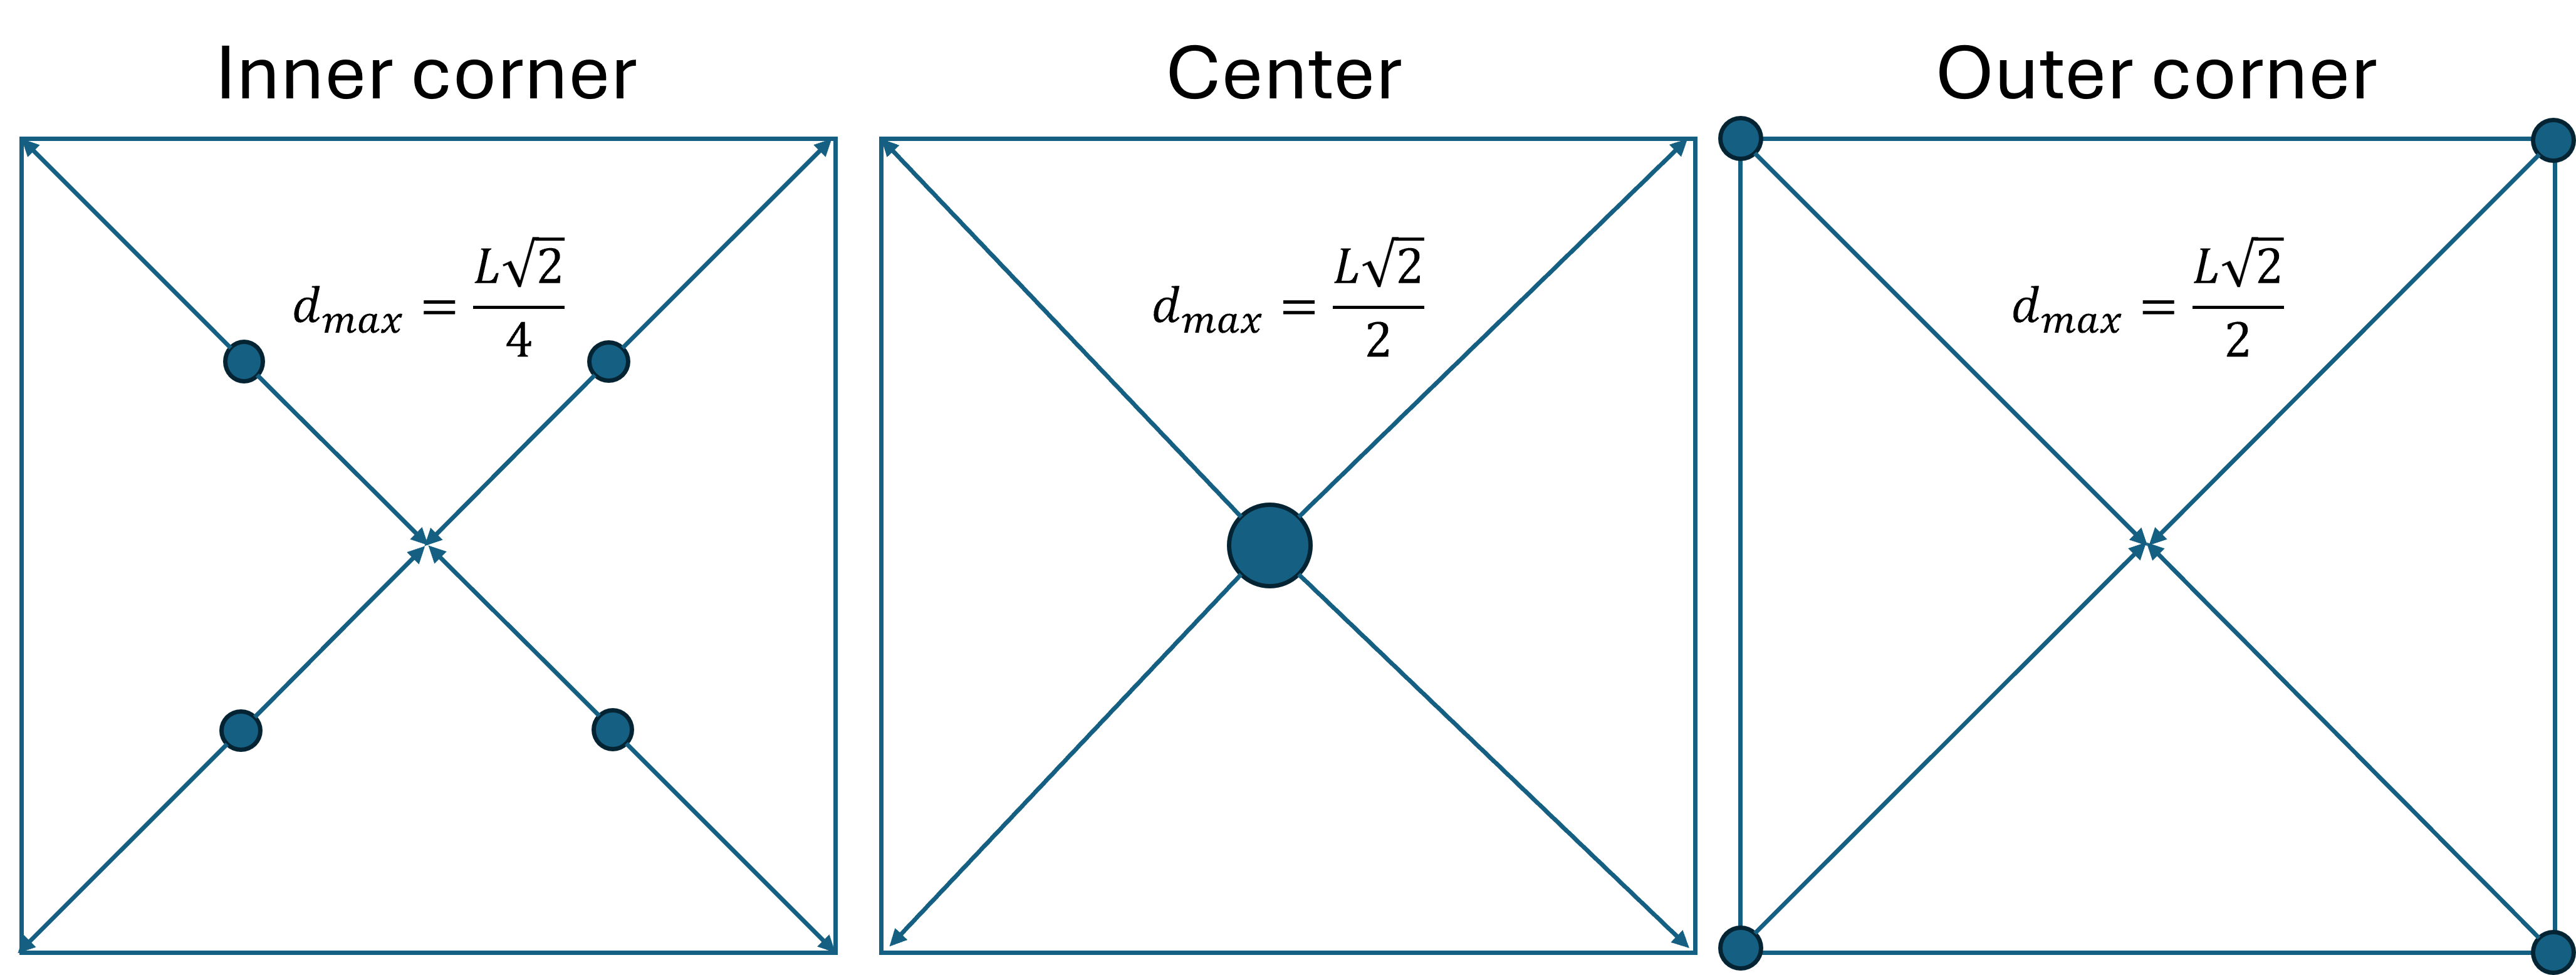
\includegraphics[width=0.8\textwidth]{figures/SA dmax.png}
    \caption{Distance $d_{max}$ of any student to a high aptitude or learned student for different seating arrangements.}
    \label{fig:SA dmax}
\end{figure}

Our analysis on the dependence of $t_{max}$ on $N$ gives us an explanation on why the traditional model performed better than the PI model in most cases. 
With lower $b$-values, the traditional model is less affected by class size than the PI models are. 
Because of this, the traditional model performed better in cases with larger classrooms. 

With regards to the performance of PI methods with traditional teaching methods, we found that classrooms with higher $\rho_0$ values performed better in PI models, while classrooms with lower $\rho_0$ values performed better in traditional models. 
A previous similar study \cite{roxas2010seating} found that classes with lower aptitude levels were the ones who benefited the most from the PI methods. 
Although we cannot directly conclude this from our model, we were able to show that students with a lower probability of learning or students who learn slower, can benefit as much from PI as in traditional set ups. 
This reinforces other studies' findings \cite{lasry2008peer} that show that PI methods can be effective even regardless of the students' actual aptitude levels.

    
